\documentclass[chapterprefix=true, 11pt, a4paper, oneside, parskip=half, listof=totoc, bibliography=totoc, numbers=noendperiod]{scrbook}

\usepackage[bottom=32mm,left=25mm,right=25mm]{geometry}

\usepackage{scrhack}

\usepackage{blindtext}

\usepackage{caption}
\usepackage{subcaption}

\usepackage{imakeidx}

\usepackage{paralist}

\usepackage{epigraph}

\usepackage[toc, acronym]{glossaries}
\glsenablehyper

\usepackage[automark,headsepline]{scrlayer-scrpage}
\automark{chapter}
\ihead{\leftmark}
\chead{}
\ohead{\thepage}
\ifoot*{}
\cfoot[\thepage]{}
\cfoot*{}
\ofoot*{}
\pagestyle{scrheadings}


\usepackage[onehalfspacing]{setspace}

\usepackage[stretch=10]{microtype}

\usepackage[english]{babel}

\usepackage{lmodern}
\usepackage[utf8]{luainputenc}
\usepackage[T1]{fontenc}

\usepackage{epigraph}

\usepackage[printonlyused]{acronym}

\usepackage{float} 

\usepackage{tabularx}

\usepackage{longtable}

\usepackage{listings}

\usepackage[table,xcdraw]{xcolor}

\usepackage{tikz}

\usepackage{graphicx}

\usepackage{wrapfig}

%\usepackage{subfigure}

\usepackage[hidelinks,english]{hyperref}

\usepackage{csquotes}
\usepackage[style=alphabetic, backend=biber, bibencoding=utf8]{biblatex}
\addbibresource{references.bib}

\usepackage{amssymb}
\usepackage{amsmath}

\addtokomafont{disposition}{\rmfamily}

\usepackage{verbatimbox}
\newcommand\Includegraphics[2][]{\addvbuffer[5pt 0pt]{\includegraphics[#1]{#2}}}

\renewcommand{\lstlistlistingname}{Source Code Content}

\renewcommand*{\labelalphaothers}{}

\renewcommand{\lstlistingname}{Code snippet}

% Create a style for system calls 
\lstdefinestyle{syscalls}{
	language=C,
	columns=fullflexible,
	aboveskip=5pt,
	belowskip=10pt,
	basicstyle=\small\ttfamily,
	commentstyle=\color{teal},
	keywordstyle=\color{blue},
	stringstyle=\color{Ao},
	showspaces=false,
	showstringspaces=false,
	showtabs=false,
	xleftmargin=16pt,
	xrightmargin=0pt,
	framesep=5pt,
	framerule=0.5pt,
	frame=single,
	rulecolor=\color{black},
	tabsize=2,
	breaklines=true,
	breakatwhitespace=true,
	captionpos=b
}

\newglossarystyle{dottedlocations}{%
	\glossarystyle{list}%
	\renewcommand*{\glossaryentryfield}[5]{%
		\item[\glsentryitem{##1}\glstarget{##1}{##2}] \emph{##3}%
		\unskip\leaders\hbox to 2.9mm{\hss.}\hfill##5}%
	\renewcommand*{\glsgroupskip}{}%
}


% Titles Config - CHOOSE ONE SECTION for title format

%% Used for titleGraduation Bachelor
%% Based on https://ai-bachelor.htw-berlin.de/files/Stg/AI/richtlinie_ba-arbeit_ai_06_02_13.pdf
\makeatletter

\renewcommand*{\maketitle}{
	\begin{titlepage}
		\newgeometry{left=2.5cm,right=2.5cm,top=2.5cm,bottom=2.5cm}
		\begin{figure}[H]
			\centering
			
\includegraphics[width=0.5\textwidth]{images/htw/logo}
		\end{figure}
		\begin{center}
			\vfill
			{\Large System Calls for Containerising and Managing Processes in Linux\par}
			\vskip 0.5cm
			{\large \bfseries A Thesis\par}
			\vskip 0.5cm
			{\large Submitted in Partial Fulfillment of the Requirements for the
                    Degree of\vskip 0.5cm \bfseries Master of Science (M.Sc.) 
                    in Applied Computer Science}
			\vskip 0.5cm
			{\large at the}
			\vskip 0.5cm
			{\large Berlin University of Applied Sciences (HTW)}
			\vfill
			\begin{flushleft}
				\begin{tabular}[t]{rl}
					First Supervisor: & Prof. Dr. Sebastian Bauer\\
					Second Supervisor: & Dr. Michael Witt \\
					Author: & B.Sc. Atanas Denkov \\
					Matriculation Number: & s0559025 \\
					Submission Date: & 04.10.2022
				\end{tabular}
			\end{flushleft}
		\end{center}
		\restoregeometry
	\end{titlepage}
}
\makeatother


\makeindex[title=Index, options=-s indexstyle.ist, intoc]
\indexsetup{level=\chapter*,toclevel=chapter}

\makenoidxglossaries
\loadglsentries{glossary.tex}
\setacronymstyle{long-short}
\begin{document}

\pagenumbering{alph} % fix for same identifier warning, character is not show in title
\maketitle

\pagenumbering{roman}
\include{chapters/preface} \clearpage 
%\include{chapter/Abstract} \clearpage
%\include{chapter/Abstract_de} \clearpage

\tableofcontents \newpage

\pagenumbering{arabic}
\chapter{Introduction}
\section{Motivation}
Primitive support for multiprocessing in the form of basic context switching and dedicated input-output 
components was introduced in the late 1950s. Multiprocessing allowed for concurrent execution of 
multiple instructions at the cost of increased system complexity. Interleaved processes had a 
global unrestricted view of the system which inevitably led to unpredictable program behaviour. 
For example, programs had the ability to modify each other's memory and monopolise 
computer resources. Hence, to ensure correctness, every program had to carefully manage its interactions 
with hardware and all other processes in the system, which resulted in an unsustainable 
programming model.

The aforementioned issues were addressed by shifting the responsibility of resource management 
and process protection into a privileged control program that acted as an intermediary between 
hardware and user programs. This program is most commonly referred to as a kernel.
The centralisation of these tasks rendered the kernel an integral part of modern computing systems. 
The kernel is an essential part of a system's trusted computing base because it acts as a 
single point of failure for all user programs. This is a particularly important issue for 
infrastructure providers that sell high-availability execution environments where 
arbitrary, and therefore, untrusted applications from different tenants coexist.
If one application tampers with the kernel, then the whole system may potentially go down. 
Similarly, 
applications are able to tamper with each other, despite the protection mechanisms enforced 
by the kernel. To solve this problem, an additional level of indirection may be introduced between the tenant program
and all other programs on the system, including the kernel, that represents an unescapable 
execution environment, also called a virtual environment.

\section{Objectives}
The primary objective of this thesis is to conduct an experiment consisting of a set of 
synthetic workloads that measure response times and efficiency within a sandboxed environment.
The experiment executes the same workloads natively, within the standard noninterference boundary 
provided by the kernel to user space programs. The differences in response times and efficiency 
within and outside a container are used as an approximation of the overhead introduced 
by isolating a process from its environment. The experiment is reproducible and can be executed 
on any Linux system with a x86\_64 or arm64 compatible processing unit.

The second objective of this thesis is to design and implement a container runtime 
that will be used by the experiment as the primary sandboxing mechanism. The runtime's 
implementation, including the system calls that it relies on, will be thoroughly discussed and its security characteristics
will be qualitatively evaluated. 

\section{Content Structure}
Chapter \ref{ch:fundamentals} introduces the fundamental axioms, or trade-offs, in virtualisation technologies.
These will be referred to throughout the entire document. 
The same chapter also introduces the concept of resource namespaces - the primary abstraction 
provided by the kernel to sandbox processes.

Chapter \ref{ch:state-of-research} outlines the current state of research in operating-system 
virtualisation, highlights the relationships between noninterference, isolation and performance, and
discusses modern architectures that try to maximise all three.     

Chapter \ref{ch:concept} provides a detailed description of the requirements and the software architecture 
of the runtime, benchmark tool, and the workloads. The measurements to be sampled from the kernel are introduced.

Chapter \ref{ch:implementation} describes the implementation of the container runtime. Furthermore,
the security characteristics of the kernel's resource namespacing capabilities are discussed.

Chapter \ref{ch:Experiment} contains the performance evaluation experiment. First, the hardware 
platform under test is discussed. Second, a set of hypotheses are developed and proven and/or 
disproven with the help of the benchmark tool.  

Chapter \ref{ch:conclusion} contains conclusive remarks, a brief summary of the results of the thesis
and future work that can be done by other students in the field.  \clearpage
\chapter{Fundamentals}
Section \ref{sections:fundamentals/virtualisation} summarises the concept of virtualisation.
Section \ref{sections:fundamentals/namespaces} introduces the concept of a namespace as defined 
in the Linux kernel and describes the individual namespace types and their effects on processes. 
Section \ref{sections:fundamentals/ebpf} presents the benchmarking tool 
that will be used to assess the performance of a namespaced application.

\section{Virtualisation}
\label{sections:fundamentals/virtualisation}
Virtualisation is the process of abstracting the execution environment of an application into 
a unit that is secure, manageable and performant. The primary value propositon of a virtualisation 
platform is the consolidation of independent and untrusted workloads onto a single 
server which cannot interfere with each other or with the host, and still exhibit optimal 
performance characteristics. Virtualisation is, in essence, a cost reduction technique for 
infrastructure providers. Unfortunately, security and performance are concepts that often conflict 
with each other, thereby rendering virtualisation into a particularly challenging domain.

Section \ref{sections:fundamentals/virtualisation/axioms} presents the fundamental axioms 
that define virtualisation - noninterference, isolation, and performance.
The first two axioms will be used to assess the security properties
that namespaces have, while the last one will be used to define a benchmark with metrics that 
measure the performance capabilities of a virtualised application. 

\subsection{Axioms}
\label{sections:fundamentals/virtualisation/axioms}
\subsubsection{Noninterference}
\label{sections:fundamentals/virtualisation/axioms/noninterference}
\textcite{10.1145/368481.368502} summarise the fundamental requirements of a multiprogramming 
system and emphasise the concept of noninterference between processes across space and time. 
\textit{Spatial noninterference} is represented by all mechanisms that protect references to memory, 
disk and input-output devices \cite{10.1145/368481.368502}. For example, memory segmentation 
is a method found in operating system kernels that assigns each process a dedicated portion
of physical memory that is invisible to all other processes in the system. The kernel traps 
any attempt made by a process to access memory outside its allocated memory segment, thereby 
guaranteeing spatial noninterference \cite{10.5555/2490781}. \textit{Temporal noninterference} refers
to those mechanisms that allocate execution time and protect against the monopolisation thereof 
\cite{10.1145/368481.368502}. For instance, CPU scheduling is a technique that decides which process 
shall run on a core such that the core does not idle and all processes make sufficient 
runtime progress \cite{10.5555/2490781}. The scheduling semantics, paired with an interrupt mechanism 
that makes sure that no process has hold of the core for too long, guarantee temporal noninterference.

\subsubsection{Isolation}
\label{sections:fundamentals/virtualisation/axioms/isolation}
\textcite{10.1145/3381052.3381315} define isolation as the level of dependency that a virtualisation 
platform has towards the host kernel. We generalise this definition and say that \textit{isolation} 
is the level of dependency that one piece of software has to another. Conceptually, isolation 
deals with explicit vertical relationships between software, and noninterference deals with 
implicit horizontal relationships between processes. Isolation can be quantified by counting the 
lines of external source code that a software executes to obtain a particular functionality. 
For example, \textcite{10.1145/3381052.3381315} count the lines of kernel code 
that a virtualisation platform executes when providing services to sandboxed applications. 
High counts indicate a strong dependency, i.e weak isolation, towards the kernel. 

\subsubsection{Performance}
\label{sections:fundamentals/virtualisation/axioms/performance}
\textcite{10.1145/3365199} defines performance as the contention between the overhead associated 
with isolating a process from its environment and the benefits of sharing resources between processes,
i.e fully utilising the capacity of the underlying resource pool. 
\textcite{10.1145/3381052.3381315} use the same definition and contrast the isolation mechanisms provided
by three different virtualisation platforms against processing unit, memory and input-output performance metrics. 
In particular, the authors define an application that computes prime numbers up to a limit. 
Since the workload is compute-bound, processing speed is measured and compared to the
number of executed lines of code that reside in the \verb|/arch|, \verb|/virt| and \verb|/arch/x86/kvm|
subsystems of the Linux kernel. \textcite{10.1145/3132747.3132763} use \textit{same-host density} as a 
performance metric that measures the number of sandboxed applications that can be consolidated onto a single server.
In addition, \textit{boot, pause and unpause times} are also considered to be important performance indicators for particular 
use cases, such as elastic content delivery networks \cite{10.1145/3050748.3050757} \cite{10.1145/3132747.3132763}
and serverless computing.

\section{Namespaces}
\label{sections:fundamentals/namespaces}
A namespace encapsulates a system resource and a collection of processes. Only processes that are 
part of the namespace can see and manipulate the resource. Namespaces are implemented in the 
kernel and are therefore a part of the trusted computing base. Container runtimes use them 
to establish a solid noninterference boundary between processes by restricting their view of the system. 
The system calls \verb|clone|, \verb|unshare|, \verb|setns| and \verb|ioctl|, as well as the 
\verb|proc| pseudo file system are the primary interaction points between a user-space program and a namespace.  

Every process is associated with a fixed-size set of namespaces, called the \textit{namespace proxy}, that corresponds to the
resources that it can access.
In user-space, the proxy is contained within the \verb|/proc/[pid]/ns| directory as a 
collection of symbolic links, each pointing to an inode number uniquely identifying a namespace 
that wraps the process identified by \verb|pid|. Currently, there are seven different types 
of namespaces reflected in the proxy. Each will be discussed individually in the upcoming sections. 

The lifecycle of a namespace is tightly coupled to the lifecycle of all processes that reside in it. 
This is reflected in how namespaces are created and destroyed. 
A namespace and a process can be atomically created via the \verb|clone()| system call.
\verb|clone()| creates a child process that begins its lifecycle by executing 
a function pointer that returns the exit code with which the child process will terminate.
In addition, the caller passes a set of configuration options that define the child's execution context.
The parent can put the child in a freshly-allocated set of namespaces by ORing a set of flags 
and injecting the result into the configuration set. It is important to note that the 
configuration set is very flexible and defines the noninterference boundary between the child and its parent. 
The parent can use it to share its virtual memory pages, file descriptor table and file system information 
with the child, thereby weakening the boundary. 
\verb|unshare()| allows an already existing process to regulate its noninterference boundary by
\enquote{disassociating parts of its execution context}. In other words, a process can 
reverse the configuration options used when it was created.
Hence, the process can detach itself into a new set of namespaces.
Alternatively, \verb|setns()| can be used by a process to join a namespace that already exists. The caller 
must have an open file descriptor referencing a namespace object from the \verb|/proc/[pid]/ns| directory. 
Notice that a namespace cannot be created without having a process to reside in it. 
A namespace is implicitly 
destroyed by the kernel when all processes inside it terminate. 
However, a user-space process can keep a namespace alive by explicitly referencing it through a 
file descriptor obtained from the proxy.

Some namespaces are represented as $n$-ary trees and can be nested up to $32$ times in order to create multiple 
noninterference boundaries. Relationships between namespaces can be queried via the \verb|ioctl|
system call that, in combination with the \verb|NS_GET_PARENT| flag, returns an initialised read-only file descriptor pointing at 
the parent namespace. 

\subsection{User namespace}
\label{sections:fundamentals/namespaces/user}
Every process is associated with a set of credentials. 
The traditional UNIX security model defines these credentials 
as a set of unique numerical user and group identifiers. The \textit{real} user and group identifiers 
represent the user to which the process belongs. They are read from the 
password database as part of the login procedure \cite{10.5555/1869911}. 
Every process spawned by the user inherits the real user and group identifiers as part of 
its credentials. 
The credentials themselves further consist of an \textit{effective} user and an effective group identifier,
which are used by the kernel to authorise and execute operations on behalf of the process \cite{10.5555/1869911}.
For example, when a process attempts to read a file, the kernel checks if the effective user ID
of the process matches the user ID of the owner of the file, or if the effective group ID matches the 
owner's group ID. If any of these predicates holds, then the effective user - and therefore the process - 
is deemed trustworthy to call the \verb|read| system call on a file descriptor referencing the file.
Typically, the effective user and group identifiers match their real counterparts. However, there 
are programs that can ambiently change the effective identifiers of a process to match 
those of the user that created them \cite{10.5555/1869911}. These programs are known as 
\textit{set-user-id} and \textit{set-group-id} programs. Every executable file is associated with 
a set-user-id and a set-group-id permission bit that can be set by that file's owner. 
If the set-user-id permission bit is set and another user executes the program, the process
obtains the effective user identifier of the file's owner, not the user that started the process \cite{10.5555/1869911}.
A classic example of a set-user-id program is \verb|sudo|, which executes arbitrary commands as the 
root user. Since the \verb|sudo| executable file is
owned by the root user and has the set-user-id bit toggled, any user cam execute any command 
in a process with full privileges. Another example is the \verb|passwd| utility which allows a user 
to change her password and therefore requires write access to the password database.  

Notice that the UNIX security model differentiates only between privileged and unprivileged processes.
The former are not subjected to permission checking and have full control of the system - they can 
reboot the system, set the system time, kill other processes and so on. 
If a set-user-id or a set-group-id program exhibits unexpected behaviour, either due to malicious manipulation or 
programming errors, this coarse-grained security model is unable to prevent a full system exploitation.
The Linux capability scheme tries to solve this problem by unbinding privileges from the root 
user and dividing them into components called \textit{capabilities}. A capability is represented as 
a single bit that is a part of a 64-bit wide bit mask, called a \textit{capability set}.
Every process is associated with a \textit{permitted}, \textit{inheritable}, \textit{effective}, 
\textit{bounding} and \textit{ambient} capability set. In this model, the effective capability 
set is used by the kernel to do permission checking. The other sets define what can be 
stored in the effective set when loading executable files that happen to also have capabilities. 
The traditional UNIX credentials, paired with the capability sets, represent a process's
security context. 

A user namespace encapsulates the security contexts of its resident processes. 
When a process creates a new user namespace, its effective user identifier
becomes the owner of the namespace and is granted full capabilities within it.
In other words, a non-privileged user on the host system can become \verb|root| within its own 
user namespace.
The kernel associates every resource and thus every other namespace type 
with a user namespace. A process is granted access to a resource in accordance with its 
credentials in the user namespace that owns the resource. 
Hence, on its own, a user namespace is not particularly useful because it does not 
own any resources. If created in pair with other namespaces, however, it becomes 
extremely useful.
\begin{lstlisting}[label={code:fundamentals/namespaces/user-example}, style=bash, caption={Example of resource ownership semantics with user namespaces}]
$ id -u && cat /proc/$$/status | grep CapEff
1000
CapEff:	0000000000000000
$ unshare -U -r  
$ id -u && cat /proc/$$/status | grep CapEff
0
CapEff:	000001ffffffffff
$ hostname mynewhostname
you must be root to change the host name
$ unshare --uts
$ hostname mynewhostname
$ hostname 
mynewhostname 
\end{lstlisting}
Example (\ref{code:fundamentals/namespaces/user-example}) highlights how the kernel authorises operations in a user namespace.
First, the security context of the current process is shown. The user running the shell has no capabilities. 
The \verb|unshare -U -r| command moves the shell into a newly-created user namespace. 
We can see that the process has obtained a superuser security context with a full effective 
capability set. Afterwards, an attempt is made to set the host name of the computer to an arbitrary string.
The operation fails, indicating that the process has insufficient privileges, even though the required 
capability is in its effective set. Why? The kernel uses an additional namespace for 
encapsulating UNIX time-sharing (uts) operations. The shell's uts namespace is owned by 
the initial user namespace, in which our user is unprivileged as shown on lines 1-3. 
To make the new user namespace useful, we encapsulate the hostname resource in a new uts namespace 
and move the shell process there. Afterwards, the kernel uses the security contexts of the new  
user namespace to authorise any UNIX time-sharing operations.

Before the advent of user namespaces,
a container runtime was required to run with superuser privileges,  
because the \verb|clone()| and \verb|unshare()| system calls require the \verb|CAP_SYS_ADMIN| 
capability. Now, if the \verb|CLONE_NEWUSER| flag is set, both system calls guarantee that the 
process will be moved in a new user namespace first, and its new security context will be used 
to authorise the creation of the remaining set of namespaces.

\subsection{Process identifier namespace}
\label{sections:fundamentals/namespaces/process}
\begin{figure}[H]
    \centering
    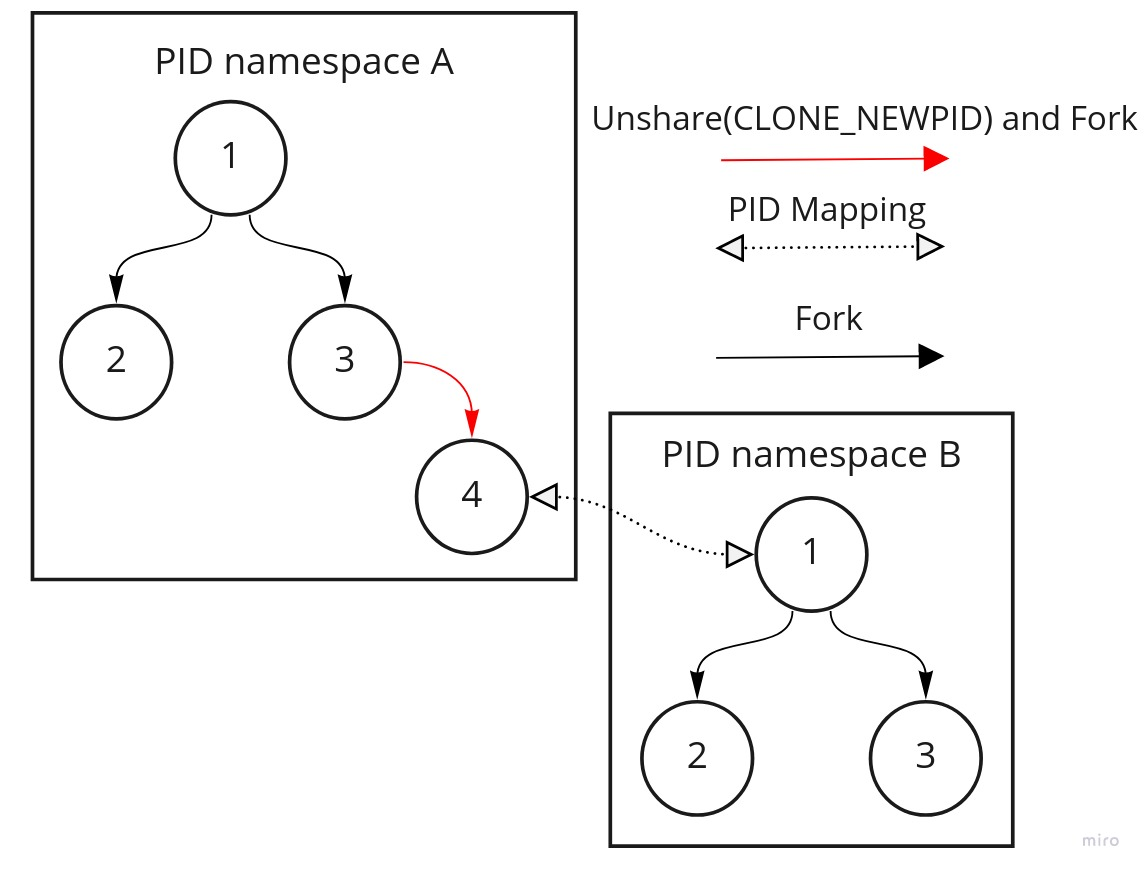
\includegraphics[width=0.55\textwidth]{images/fundamentals/pid-namespace-hierarchy.jpg}
    \caption{PID namespace hierarchy}
    \label{images:fundamentals/pid-namespace-hierarchy.jpg}
\end{figure}
Process identiifer (PID) namespaces encapsulate the mechanism of assigning 
unique identifiers to their resident processes. Every PID namespace localises an associative 
array, called the identifier registry, capable of allocating up to $2^{22}$ unique numbers and mapping them to arbitrary 
pointers. Because of this localisation, processes in different namespaces can be mapped to the 
same identifier. The first process to join a PID namespace receives the process identifier $1$ 
and acts as the init process for the entire namespace. This process becomes the parent of 
any orphaned children inside the namespace. Furthermore, if the init process terminates, all processes 
in the namespace terminate as well. In this case, even if a file descriptor to the namespace is kept open, 
i.e the namespace is kept alive by the kernel, no process is allowed to join.  

Process identifier namespaces are organised into a hierarchy, 
as shown by Figure (\ref{images:fundamentals/pid-namespace-hierarchy.jpg}).
When a process calls \verb|unshare| with the \verb|CLONE_NEWPID| flag set, 
the kernel does not detach the process into a new PID namespace. Doing so would require 
changing the identifier of the process.
Instead, the kernel caches the new namespace in the process's namespace proxy and 
spawns the process's future children into it. The new process namespace is accessible from 
user-space via the \verb|/proc/[pid]/ns/pid_for_children| file. 

We denote $N_{i}$ as the $i$-th process in namespace $N$. 
In Figure (\ref{images:fundamentals/pid-namespace-hierarchy.jpg}),
$A_{1}$ forks two children $A_{2}$ and $A_{3}$. 
$A_{3}$ calls \verb|unshare| and registers a new PID namespace in the kernel. The process 
subsequently forks $A_{4}$, which the kernel translates into $B_{1}$.
Note that $A_{1}$ and $A_{2}$ can, by definition, interact with $B_{1}$ because $B_{1} = A_{4}$.  
Hence, a process is visible to all of its peers in its namespace and to all direct ancestor
namespaces. Conversely, $B_{2}$ and $B_{3}$ cannot see any processes in $A$. 
Joining a PID namespace is an irrevirtible operation, i.e if $A_{2}$ joins $B$,
then it cannot go back.

PID namespaces can be nested arbitrarily up to 32 times. 
Container runtimes do not utilise this feature, because application workloads are orthogonal 
to each other. Nesting two application workloads, potentially stemming from two different tenants, in a hierarchy
would enable processes resident in the ancestor namespace to kill the init process of the child namespace, which 
is in direct conflict with the noninterference property. 

\begin{lstlisting}[style=c-code-snippets, label={code:fundamentals/namespaces/process}, caption={PID namespace creation pseudocode}]
/* pid_namespace.c */
int err = unshare(CLONE_NEWPID);
pid_t child = fork();
if (child == 0) 
    child = fork();
    if (child == 0)
        execlp("sleep", "sleep", "60", (char *) NULL);
    else if (child > 0)
        exit(waitpid(child, NULL, 0) != child);
else 
    return waitpid(child, NULL, 0) != child;
\end{lstlisting}

Code snippet (\ref{code:fundamentals/namespaces/process}) demonstrates the creation of a new 
PID namespace with two processes. On lines 1 and 2, a new 
pid namespace is created through the \verb|unshare| system call and its init process is forked. 
The init process creates a new child that sleeps for 60 seconds. All processes within this 
hierarchy await their children's completion. 
We can run this example in a shell and list the shell's children via the \verb|ps|
utility, as shown in Code snippet (\ref{code:fundamentals/namespaces/process-cmd}). 
You'll notice that the \verb|sleep| command is visible from the ancestor namespace and can be killed,
i.e directly interfered with. 
\begin{lstlisting}[label={code:fundamentals/namespaces/process-cmd}, style=bash, caption={Example of creating a PID namespace and listing all processes in the child namespace from a process in the parent namespace}]
$ ./pid-namespace &
[1] 78972
$ ps
PID TTY TIME CMD
62983 pts/1 00:00:00 bash
78972 pts/1 00:00:00 pid-namespace
78973 pts/1 00:00:00 pid-namespace
78974 pts/1 00:00:00 sleep
79027 pts/1 00:00:00 ps
\end{lstlisting}

%This has several implications. First, 
%this process becomes the parent of any orphaned children.
%If it fails to reap a child, the kernel will not release the child's process identifier from 
%the namespace identifier registry. Cumulatively pilling up the reserved identifiers may 
%result in the inability to spawn new processes. Second, if the init process terminates, all 
%processes in the namespace are terminated as well. 

%The noninterference boundary of a PID namespace heavily relies on the correct operation of the 
%init process. To prevent a member of the PID namespace from killing the init process and therefore 
%interfering with its peers, the kernel only propagates signals for which the init process 
%has established handlers for. 

\subsection{Mount Namespace}
\label{sections:fundamentals/namespaces/mount}
\begin{table}[h!]
    \centering
    \begin{tabular}{ |m{4cm}|m{20em}| }
        \hline
        Propagation Type & Description \\
        \hline
        \verb|MS_SHARED| & Mount and umount events are propagated across mount namespaces. \\
        \hline 
        \verb|MS_PRIVATE| & Mount and umount events are local. The mount point does not propagate, nor does it receive mount and umount events. \\
        \hline
        \verb|MS_SLAVE| & Mount and umount events are propagated unidirectionally from a master set of mount points to a slave mount. \\
        \hline
        \verb|MS_UNBINDABLE| & Mount point is private and cannot be bind mounted \\
        \hline
    \end{tabular}
    \caption{Table of mount point propagation types in Linux}
    \label{table:fundamentals/namespaces/mount/propagation-types}
\end{table}

Files are multiplexed across multiple devices, each with its own intrinsic implementation details 
for storing and managing data. The kernel abstracts the underlying idiosyncrasies 
by arranging all files into a hierarchy that can be accessed through a well-defined programming interface. 
The process of attaching a device's file system 
to this hierarchy is called \textit{mounting}. The position in the hierarchy where the file system 
is attached is referred to as a \textit{mount point}.

Mount namespaces encapsulate the list of mount points that their resident processes can 
see. When a process detaches into a new mount namespace, it inherits an exact replica of the parent's mount points.
This does not necessarily mean that a change made by the parent to an underlying mount point remains 
invisible to the child, or vice versa. Every mount point is associated with a dedicated \textit{propagation type} 
that determines whether or not mount and umount events are shared across mount namespaces 
that reference it or any mount points immediately below it in the file hierarchy.  
In essence, the propagation type governs the file system's noninterference boundary. 
Table (\ref{table:fundamentals/namespaces/mount/propagation-types}) summarises the possible 
propagation types. The \verb|/proc/self/mountinfo| file 
displays a multitude of mount point properties with respect to the mount namespace in which 
the process reading the file resides in. 

In addition to mounting device file systems onto the file hierarchy, we can make 
already mounted subtrees visible at other locations in it. This concept is known as a 
\textit{bind mount}. Bind mounts are commonly used by container engines to map directories 
on the host system to directories inside a container. Internally, the kernel copies
the data structures of the original mount into a new mount point inside 
container's mount namespace. Changes in one mount point are reflected in the other 
using copy on write. 

\subsection{Network Namespace}
\label{sections:fundamentals/namespaces/network}
\begin{figure}[H]
    \centering
    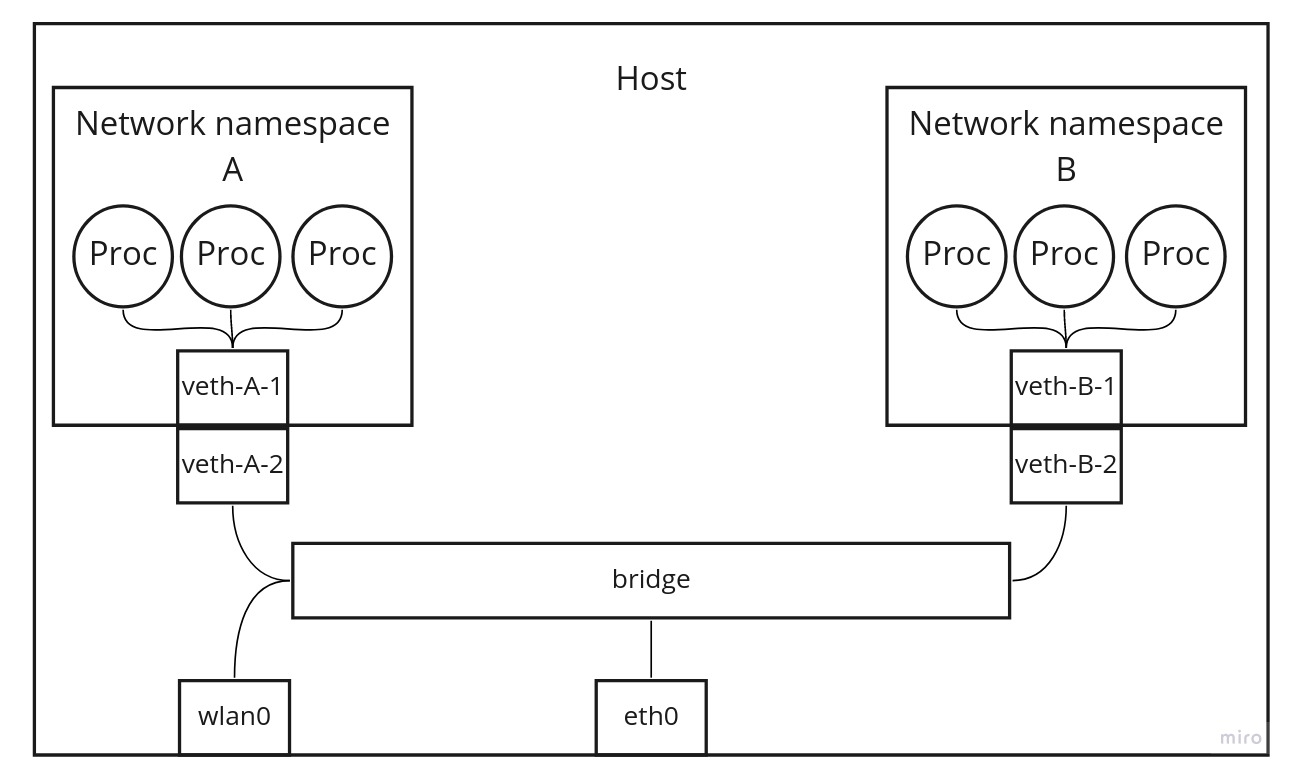
\includegraphics[width=0.65\textwidth]{images/fundamentals/net-ns-veth-arch.jpg}
    \caption{Network architecture that enables inter-container communication via bridge and virtual ethernet devices.}
    \label{images:fundamentals/net-ns-veth-arch.jpg}
\end{figure}

Network namespaces encapsulate the full network stack and expose it only to 
their resident processes. This allows a collection of processes to operate on 
dedicated network interfaces, routing tables, firewall rules and UNIX domain sockets 
that are inaccessible to others. 

The kernel imposes an important restriction. A physical network device can be attached only 
to a single network namespace. When the network namespace is released, the phyiscal device 
is returned back to the initial network namespace, i.e the host. To enable socket-based interprocess
communication across network namespace boundaries, 
the physical devices need to be multiplexed on top of virtual interfaces. 

All container engines implement the same default network configuration that allows processes 
in different network namespaces to communicate with each other. As part of its initialisation procedure,
the container engine installs a bridge interface inside the root network namespace.
A bridge can be thought of as a virtual network switch. 
It forwards packets between interfaces, called slaves, that are attached to it. 
Before detaching a process into a new network namespace, the container engine creates a 
virtual ethernet device. Virtual ethernet devices are a software equivalent of a patch cable. 
They are represented by a pair of interconnected endpoints. One end of the virtual ethernet device is moved 
into the network namespace of the process, and the other remains on the host and is attached 
to the bridge. Because the bridge acts as a switch, other network devices attached 
to it can communicate with a namespaced process. Figure (\ref{images:fundamentals/net-ns-veth-arch.jpg})
visualises such a network configuration. In it, two network namespaces, and a wlan interface
inside the root namespace, can exchange data over the bridge. Code snippet (\ref{code:fundamentals/namespaces/network-example})
shows how to configure such a network.
\clearpage

\begin{lstlisting}[label={code:fundamentals/namespaces/network-example}, style=bash, caption={Commands for configuring the network as shown in  Figure (\ref{images:fundamentals/net-ns-veth-arch.jpg})}]
$ ip netns add A 
$ ip netns add B 
$ ip link add veth-A-1 netns A type veth peer name veth-A-2
$ ip link add veth-B-1 netns B type veth peer name veth-B-2
$ ip netns exec A ip addr add "192.168.1.1/24" dev veth-A-1 
$ ip netns exec B ip addr add "192.168.1.2/24" dev veth-B-1
$ ip netns exec A ip link set veth-A-1 up 
$ ip netns exec B ip link set veth-B-1 up 
$ ip link set veth-A-2 up 
$ ip link set veth-B-2 up 
$ ip link add name br-AB-0 type bridge 
$ ip link set br-AB-0 up 
$ ip link set veth-A-2 master br-AB-0 
$ ip link set veth-B-2 master br-AB-0 
$ ip addr add 192.168.1.10/24 brd 192.168.1.255 dev br-AB-0
\end{lstlisting}

On lines 1-2, two network namespaces $A$ and $B$ are created. On line 3, a virtual ethernet 
cable is created, whose ends are represented by \verb|veth-A-1| and \verb|veth-A-2|. The former 
is injected into namespace $A$, whilst the latter is kept in the root namespace. 
The same process is executed on line 4 for namespace $B$. The isolated ends of the 
virtual devices are initialised and assigned unique IP addresses that are a part of the same logical network.
The other ends are initialised as well. On lines 11-14 a bridge is created and the 
virtual ethernet cables are attached to it. At this point, $A$ and $B$ can communicate 
effectively with each other. The host, however, interprets the bridge solely as an L2 packet 
forwarder that cannot interact with the other namespaces. On line 15, the bridge
is made a participant of the isolated network by being assigned an IP address.
Now, both namespaces and the host can communicate with each other. 
However, a mechanism for routing traffic from the bridge to a different node in the 
host network or the internet is missing. 

\subsection{Interprocess Communication Namespace}
\label{sections:fundamentals/namespaces/ipc}

\subsection{UNIX Time-Sharing Namespace}
\label{sections:fundamentals/namespaces/uts}
UNIX Time-Sharing (uts) namespaces encapsulate the system's host name and domain name.
When creating a new uts namespace, the kernel simply copies the system identifiers of the 
previous namespace and exposes the copied versions to all residents of the namespace. 
The residents are free to change both identifiers without affecting the actual values 
on the host. Example (\ref{code:fundamentals/namespaces/user-example}) already highlights 
how to detach a shell into a new uts namespace and set its host name.

\subsection{Control Group Namespace}
\label{sections:fundamentals/namespaces/cgroups}

\section{Extended Berkley Packet Filters (eBPF)}
\label{sections:fundamentals/ebpf} \clearpage
\chapter{State of research}
\label{ch:state-of-research}
\textit{Operating system virtualisation} refers to all mechanisms that enable the creation of secure
and isolated application environments that run on top of a shared kernel. 
Conventionally, these mechanisms are baked into the kernel and are therefore part of the trusted computing base.
The kernel may expose these through its system-call interface, thereby allowing a user-space daemon 
program to provide an automated facility for creating and orchestrating sandboxed environments. 
This is the only feasible architecture on a general-purpose kernel such as Linux. 
Alternatively, the kernel may treat every software component, including its own subsystems, as an entity
to be wrapped in a sandbox. In that case, the concept of a process itself would have to 
satisfy all three virtualisation axioms. Examples of such operating systems include the seL4 \textit{microkernel}
- the first operating system to be formally verified as free of programming errors \cite{10.1145/1629575.1629596}, 
and Google's Fuchsia - described by \textcite{10.22667/JOWUA.2021.09.30.047}.

An application, referred to as a \textit{container},
is defined as an encapsulation of \enquote{[...] a software component and all its dependencies 
in a format that is self-describing and portable, so that any compliant container runtime can run it without extra 
dependencies, regardless of the underlying machine and the contents of the container} \cite[1]{oci-runtime-principles}.
A \textit{container runtime} is the user-space daemon program responsible for bringing this portable but 
static representation of an application into execution. In runtime, a container consists of a collection of processes 
that share a restricted view of the system's resources. For example, every container \enquote{believes}
it has a dedicated network stack with its own network interfaces, routing tables and packet-forwarding rules.
All processes in the container can access and manipulate that network stack, but no other process 
outside the container has that capability.
The container runtime configures this invariant and the operating system enforces it by 
namespacing system resources. The Open Containers Initiative (OCI) \cite{oci-website} has 
developed a runtime specification that standardises the operations a container runtime
needs to support. Most importantly, it must allow an external process called a \textit{container engine}
to hook into the lifecycle of a container. The container engine can use these hooks to manage 
all the containers on a single host system. In addition, the engine can attach network and storage 
to containers, thereby allowing processes in different sandboxes to share state and communicate 
with each other, if required. At the highest level of abstraction sits an orchestration platform that 
manages containers on multiple hosts by interacting with the container engine on each system.
This platform constantly monitors node and container health and dynamically multiplexes workloads 
based on various system properties of the cluster as to ensure maximum application availability.

It is important to note that, by definition, the kernel is assumed to be trustworthy. 
It has full control of all hardware resources and can access and modify the execution environment of every process on the system. 
In other words, noninterference between the kernel and user processes is not guaranteed.
Therefore, if the kernel is compromised, all processes on the system become untrustworthy.
It follows that if a process compromises the kernel, it transitively interferes with all other 
processes on the system. Hardening the operating system by implementing various security features such as
mandatory access control has been the primary approach for protection against such scenarios. 
However, the size of a monolithic general-purpose kernel is too large to adequately 
create a threat model that captures all possible vectors of attack. This problem is of particular concern 
to infrastructure providers whose entire business model revolves around consolidating hundreds of potentially 
malicious client applications on the same server, all of which share the same kernel and are allowed to directly interact with 
it via its system call interface. 

Unlike hardware virtualisation, this architecture does not use hardware emulation as an 
isolation primitive.
This means that shadow pages need not be maintained per virtual environment. Input-output operations need only 
traverse the kernel's stack without any address translations and with the additional 
performance benefit of direct memory access. As a result, the isolation overhead is lower 
compared to a virtual machine, which allows more applications to be consolidated onto a single server.
Furthermore, guests do not boot up complete operating system images, which reduces 
start times and memory consumption.
\textcite{10.1145/3126908.3126925} use containers in high-performance 
computing clusters to run user-defined compute jobs and show that the imposed performance penalties 
are, at most, negligible compared to vanilla processes that have no additional isolation.
\textcite{7095802} show the exact same thing and further conclude that the Docker container engine 
is resource-friendlier and faster than the Kernel Virtual Machine (KVM) when stressing the
\enquote{memory, IPC, network and filesystem subsystems} \textcite[1]{7095802} of the Linux kernel 
by running a database inside a virtual environment and evaulating its performance via the SysBench OLTP benchmark \cite{sysbench-oltp}.

Google's gVisor \cite{google-gvisor} attempts to sustain the performance advantages of 
containers whilst introducing an additional isolation boundary between the kernel and each container. The authors implement 
a substantial portion of the system call interface in a user-space process called Sentry.
Their dedicated container runtime calls out to Sentry instead of the kernel when issuing system calls.
\begin{figure}[H]
    \centering
    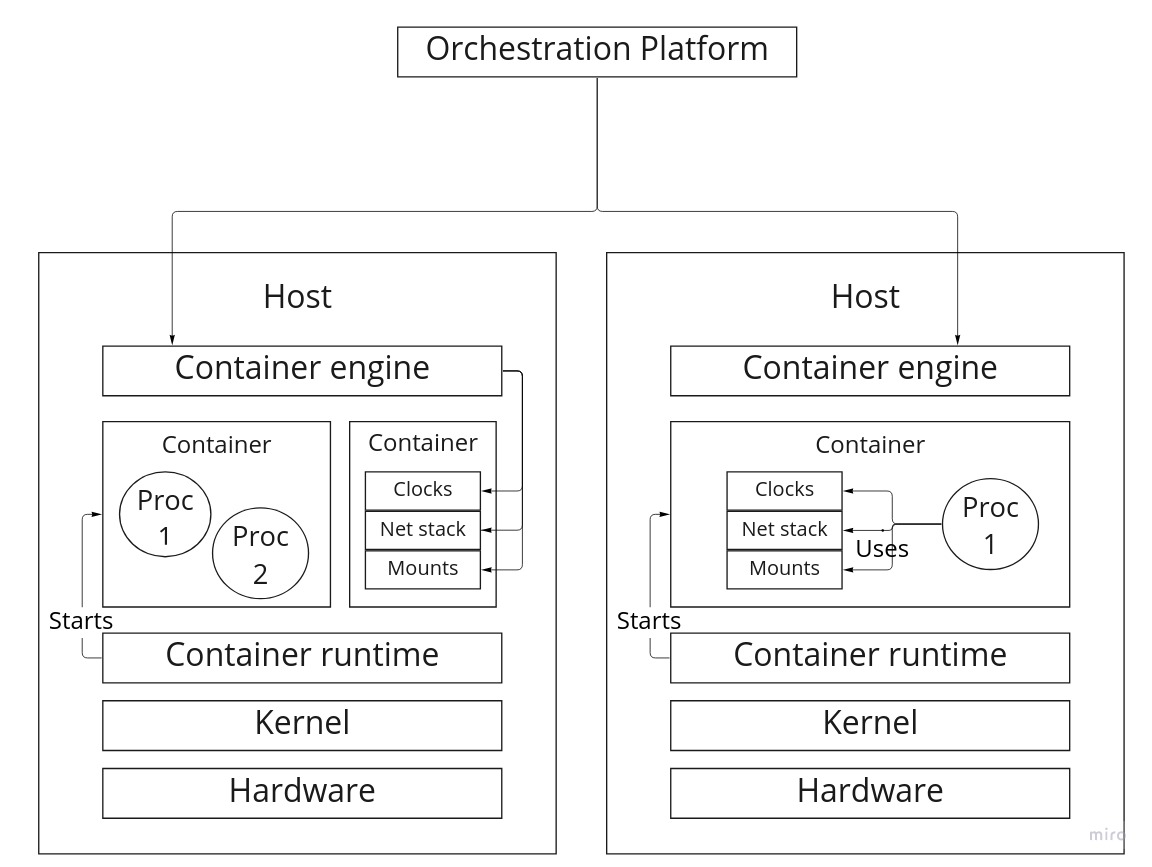
\includegraphics[width=0.55\textwidth]{images/fundamentals/cont-arch.jpg}
    \caption{Operating system virtualisation architecture using containers. The container runtime starts containers on a single host.
    A user process can see a bundle of resources allocated to it by the kernel. The kernel guarantees that a process 
    cannot see any other resources.
    The container engine manages all containers on a single system and allocates storage and networking to create explicit paths between containers.
    The orchestration platform talks to all engines inside a cluster to provide automatic workload management.}
    \label{images:fundamentals/cont-arch.jpg}
\end{figure}
However, \textcite{234857} show that network and memory allocation performance greatly suffer. 
This can be partially attributed to the fact that the Sentry process is implemented in a garbage-collected language 
and lacks the fine-grained optimisations contained in the Linux kernel.
\textcite{246288} take a different approach and try to fuse the security of virtual machines 
with the performance of containers by programming a custom virtual machine monitor 
called Firecracker that runs on top of KVM. Firecracker completely relies on the
Linux kernel for memory management, CPU scheduling and block I/O. To reduce its attack surface,
the virtual machine monitor sacrifices portability by supporting a limited set of emulated 
network and block devices. To further strengthen the noninterference boundary, the devices 
have configurable built-in rate limiters that can control the number of operations per second, e.g
disk/packets per second. Unlike a traditional container runtime, Firecracker's rate-limiting implementation
does not rely on the kernel, which makes its isolation boundary to the kernel stronger. 
\textcite{10.1145/3381052.3381315} evaluate both gVisor and Firecracker and show that 
the latter \enquote{[...] is effective at reducing the frequency of kernel code invocations, but had 
a much smaller impact on reducing the footprint of kernel code} \cite[12]{10.1145/3381052.3381315}. 

\textcite{10.1145/361011.361073} refer to the control program as a \textit{virtual machine monitor} that 
ensures isolation and noninterference by providing every program with an environment that is \enquote{[...] effect
identical with that demonstrated if the program had been run on the original machine directly} 
\cite[2]{10.1145/361011.361073}. This definition implies that a running program does not directly use
the bare metal resources available. Instead, resources are emulated by the virtual machine monitor at
the hardware level and presented as a dedicated physical system. Such an environment is called 
a \textit{virtual machine}.

\begin{figure}[H]
    \centering
    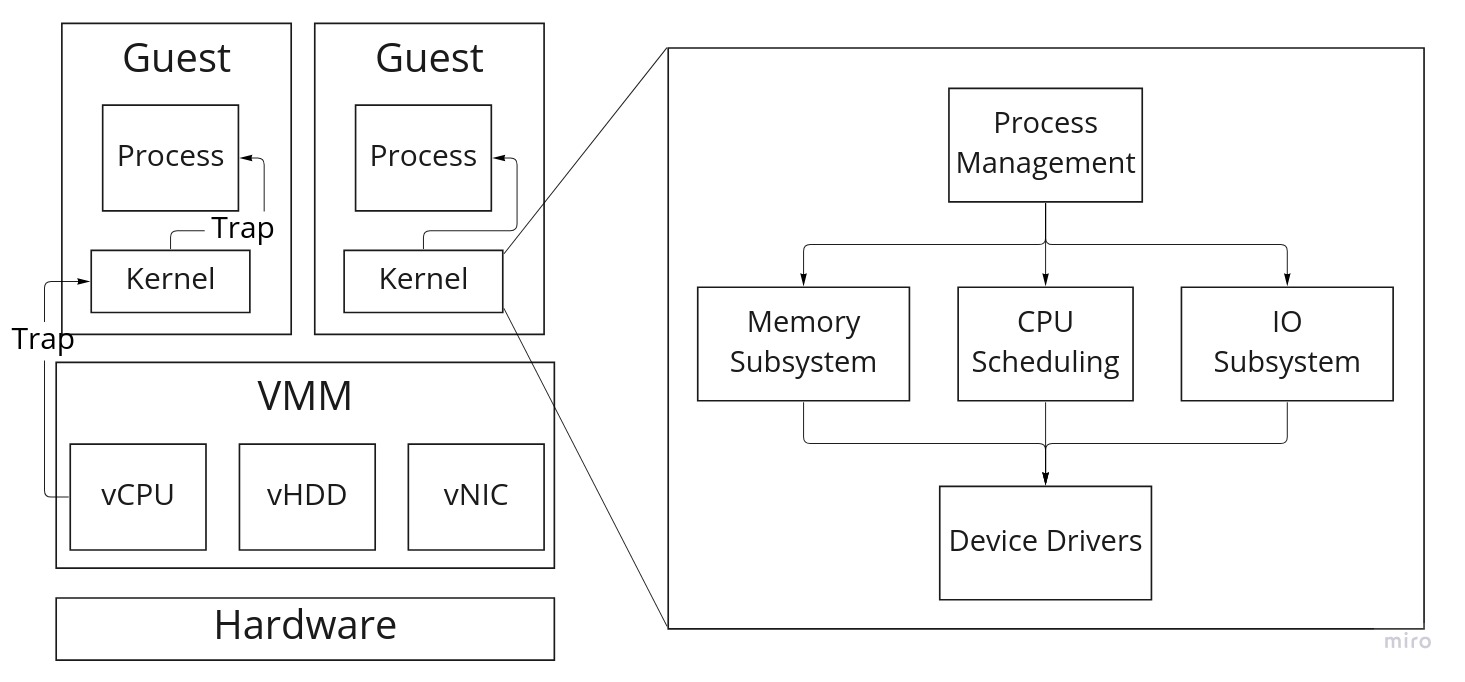
\includegraphics[width=0.70\textwidth]{images/fundamentals/full-virt-archh.jpg}
    \caption{Hardware virtualisation architecture. Each guest runs a complete operating system. 
             Privileged operations are trapped by the virtual machine monitor and emulated to provide hardware services.}
    \label{images:fundamentals/full-virt-archh.jpg}
\end{figure}

\textcite{10.1145/361011.361073} define a requirement that the instruction-set architecture of a computer
has to satisfy for it to be virtualisable. The instruction set must be segregated into three groups of
instructions - privileged, sensitive and innocuous. An instruction is privileged if it requires changing
the mode of execution from user to supervisor mode by means of a trap \cite{10.1145/361011.361073}. 
An instruction $i$ is control-sensitive if, when applied to the current processor state $S_1$, results
in a new state $i(S_{1}) = S_{2}$ such that the execution mode of $S_{2}$ does not equal that of $S_{1}$
or if $S_{2}$ has access to different resources than $S_1$ or both \cite{10.1145/361011.361073}. 
An instruction is behaviour-sensitive if its execution depends on the execution mode or its position
in memory \cite{10.1145/361011.361073}. An instruction is innocuous if it is not sensitive. 
Given these definitions, a computer is virtualisable \enquote{[...] if the set of sensitive instructions
for that computer is a subset of the set of privileged instructions} \cite[6]{10.1145/361011.361073}.
If this criterion is met, the virtual machine monitor can trap all sensitive instructions and emulate 
each via a homomorphism $i: C_{r} \rightarrow C_{v}$ that maps the state space of the processor without
the virtual machine monitor loaded $C_{r}$ to the state space with the virtual machine monitor loaded 
$C_{v}$ \cite{10.1145/361011.361073}. Innocuous instructions do not require protection, i.e a homomorphic
mapping, and are directly executed by the processor \cite{10.1145/361011.361073}.

Given the aforementioned homomorphism, a virtual machine can host a \textit{guest kernel} (Figure \ref{images:fundamentals/full-virt-archh.jpg}) that 
runs completely in user mode. 
Whenever the guest kernel attempts to execute a privileged instruction, 
the virtual machine monitor traps the attempt and emulates the instruction. 
Consequently, the guest kernel does not have to be a part of the trusted computing base. 
Even if it is compromised or encounters an unrecoverable error condition, other virtual machines 
remain unaffected. As a result, the isolation boundary between user programs running in different 
virtual machines is stronger compared to processes running on a shared kernel. 

In order to fully guarantee spatial noninterference between processes, the virtual machine monitor must 
be in full control of the host system's memory. There are two primary methods to do this - 
\textit{shadow paging} and \textit{extended page tables}. The former mechanism is considered first. 
The virtual machine monitor maintains a nested page table 
per guest, also called a \textit{shadow page table} \cite{10.5555/1204009}. 
In turn, the guest kernel maintains a page table per process. 
Whenever the guest kernel schedules a new process for execution, it modifies the \textit{page-table 
base register} to point to the page table for that process \cite{10.5555/1204009}. 
The virtual machine monitor intercepts this attempt and transparently updates the page table pointer to point to 
the guest's shadow page table corresponding to that process \cite{10.5555/1204009}. Note that 
the virtual machine monitor has to traverse the shadow page table for that guest in order to find the nested entry corresponding 
to the process. Afterwards, the memory management unit takes care of translating the virtual memory 
addresses of the guest and updating the \textit{translation lookaside buffer}.
Alternatively, the memory management unit may be \enquote{virtualisation-aware} in the sense that it knows 
there are two page tables it needs to traverse - the page table that maps guest virtual memory to guest 
\enquote{physical memory}, and the page table that maps guest physical memory to actual physical memory. 
The former is maintained by the guest kernel, whilst the latter is maintained by the virtual machine monitor.
The extended page table approach is up to 50\% faster than shadow paging \cite{2006PerformanceEO} because table
walks are done in hardware - by the memory management unit.
Nevertheless, maintaining page table data structures inside the virtual machine 
monitor and the guests leads to memory pressure, which is further amplified by the fact that 
guests, their applications and the virtual machine monitor all share the same physical memory \cite{10.5555/2490781}. 

The spatial noninterference property necessitates that the virtual machine monitor manage 
all input-output devices and their interactions with the guests. This is accomplished by the
already introduced trap-and-emulate pattern. When an application within a virtual machine 
issues a system call requesting some form of input-output, the request is processed by the 
I/O stack inside the guest. At the lowest level of the stack, the device driver issues a 
command to the device, typically by writing to memory specifically assigned to the device, or by
calling specific input-output instructions \cite{10.5555/2490781}. 
Either way, the virtual machine monitor intercepts this and traverses its own I/O stack, which 
remaps guest and real input-output addresses and forwards the request to a physical device \cite{10.1145/2063176.2063194}. 
After processing the request, the physical device triggers an interrupt that is caught by the virtual machine monitor and 
transformed into a virtual equivalent that is sent to the virtual machine that issued the request.
To reduce the overhead associated with interrupt processing, the virtual machine monitor can batch 
multiple events together and use a single interrupt to notify the guest kernel \cite{10.1145/2063176.2063194}.
Still, a request must traverse two input-output stacks. The same holds for the response.
In addition, hardware optimisations such as direct memory access are emulated in software, which 
further degrades performance. This, however, can be mitigated by integrating an input-output memory management 
unit that remaps all direct memory accesses of a device on the host to an address space in the guest.

The cost of hardware virtualisation becomes apparent when measuring same-host density
and boot times. \textcite{10.1145/3132747.3132763} consider memory consumption and on-disk image size
as the primary limiting factors. The authors measure the time it takes to create and boot
virtual machines using the Xen virtual machine monitor and show the negative effects that on-disk image size has 
by starting images with 
varying sizes by manually \enquote{[...] injecting binary objects into the uncompressed image file} \cite[3]{10.1145/3132747.3132763}. 
As the number of consolidated virtual instances increases and the image size grows, 
creation and boot times increase linearly.
Furthermore, the authors show that creating and starting a process directly on the host is, on average, 
two orders of magnitude faster. \textcite{10.1145/2151024.2151030} also evaluate Xen and state
that processing units spend 25\% of their total cycles in hypervisor mode instead of executing guest applications 
when running \enquote{[...] SPEC's first benchmark addressing performance evaluation of datacenter servers used in 
virtualised server consolidation} \cite[2]{10.1145/2151024.2151030}, which includes components 
such as a web, database and application server.
 \clearpage
\chapter{Concept}
\label{ch:concept}
This chapter introduces the functional and non-functional requirements of two 
applications - the container runtime and the benchmarking tool. 
In addition, architectural diagrams are provided and discussed. 
Example usage of both applications is shown.
This chapter also contains a thorough justification of the workloads deployed by the benchmarking tool as
well as the variables used to measure the performance of the sandboxed workloads.

\section{Container runtime}
The container runtime is the component responsible for wrapping a user-defined binary 
in a sandbox. It will be used by the benchmarking tool to wrap workloads in sandboxes.

\subsection{Functional requirements}
The Open Containers Initiative standardises the operations \cite{oci-runtime-operations} that 
a container runtime needs to support.

\begin{enumerate}[i]
\item The container runtime must provide clients with state information for a container
given its unique identifier. 
\label{requirements:container-runtime/1}
\item The container runtime must provide clients with the ability to create a new container. 
Users must supply the runtime with a unique identifier for the container and a path to a 
container bundle. The latter consists of a root filesystem and a configuration file that 
defines, amongst other things, the path to the user-defined binary and the set of namespaces
it will reside in.
\label{requirements:container-runtime/2}
\item The container runtime must provide clients with the ability to start a container. 
Users must provide the unique identifier of the container to start. 
This operation must execute the user-defined binary in the sandboxed environment.
\label{requirements:container-runtime/3}
\item The container runtime must allow users to kill the container process.
Users are required to provide the unique identifier of the container and the signal to be sent 
to the container.
\label{requirements:container-runtime/4}
\item The container runtime must allow users to delete the container.
The delete operation must remove all resources allocated in (\ref{requirements:container-runtime/2})
\label{requirements:container-runtime/5}
\item The container runtime must allow external applications to hook into well-defined points 
of a container's lifecycle.
\label{requirements:container-runtime/6}
\end{enumerate}

It is important to note that the container runtime's only responsibility is to sandbox processes. 
An external application, such as the benchmarking tool discussed later, 
must have the ability to interact with the runtime for the purpose of configuring 
the sandboxed environment. This includes operations such as creating network topologies that interconnect 
different containers or allocating shared filesystems. From this, requirement 
(\ref{requirements:container-runtime/6}) has been derived. 

\subsection{Non-functional requirements}
All requirements specified in this section are ranked in order of importance. 
\begin{enumerate}[i]
\item The container runtime must not pollute or damage the host system via its operation.
The runtime manages sensible resources, such as mount points and devices. It must in no way 
cause side effects on the host, leading to operational failure. This is also an important factor 
for allowing reproducibility of the work. Users must be able to use the runtime without fear of 
damaging their system. 
\label{requirements:non-functional/container-runtime/1}
\item The container runtime must support unprivileged containers, i.e containers that run without 
root privileges on the host system. This is in and of itself a functional requirement for running 
containers in multitenant environments. 
\label{requirements:non-functional/container-runtime/2} 
\item The container runtime must be implemented in a programming language with manual memory management.
Satisfying this requirement will ensure that future work aimed at measuring container boot times 
will not be hindered by unpredictable perturbations introduced by a garbage collector.
\label{requirements:non-functional/container-runtime/3}
\item The container runtime must consist of a library component and an executable component. 
This will allow users to implement their own abstractions on top of the library for other research-related 
purposes. 
\end{enumerate}

\subsection{Architecture}
\label{ch:concept/runtime/architecture}
\begin{figure}[H]
    \centering
    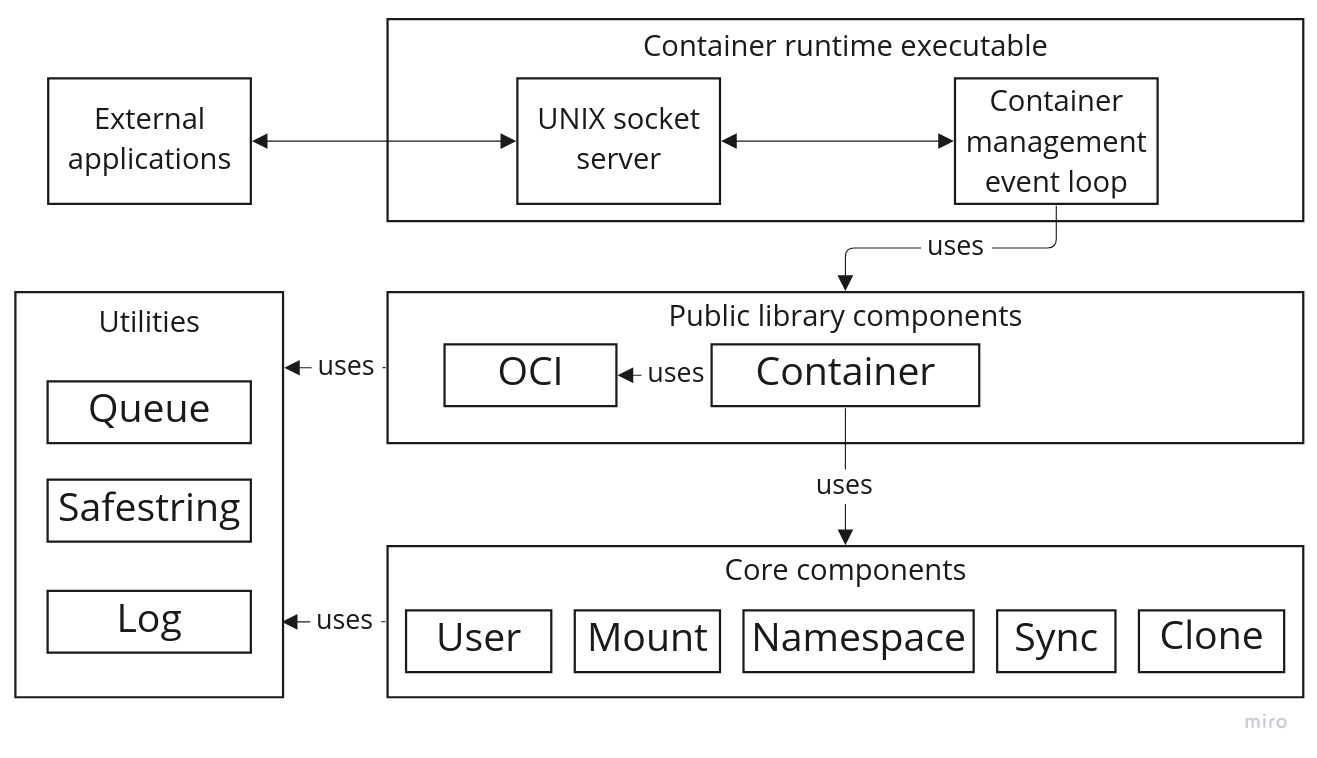
\includegraphics[width=0.55\textwidth]{images/concept/runtime-arch-overview.jpg}
    \caption{High-level overview of the runtime architecture}
    \label{images:concept/runtime-arch-overview.jpg}
\end{figure}
The architecture of the runtime is shown in Figure \ref{images:concept/runtime-arch-overview.jpg}.
It consists of a library and an executable that uses it to provide container 
management services to external applications. The library is split into three parts - utilities,
core components and public components. 

The utilities provide common data structures such as 
linked lists and queues. They also contain procedures for safe string manipulation, a logger,
and a multitude of helper macros that enable the safe management of resources such as file descriptors 
and heap memory. The core components directly interface with the kernel. 
They are responsible for configuring the container, 
i.e the execution environment of the user-defined application. On top, the public library 
components use the core components to provide a 
simple interface for creating, starting, killing and deleting containers. A container 
is represented as an opaque pointer and is only allowed to be accessed through library functions.

The runtime executable uses the container component to create and manage a single container.
It consists of an event loop that monitors state changes of the container and reaps the process 
when it exits. In addition, it polls a signal file descriptor for itself. When the user desides 
to kill the runtime executable, the same signal is propagated to the container, the container 
is killed, and all resources it allocated are deleted accordingly. 

When a process is detached into a new user namespace, it's real user identifier is replaced by the kernel 
with the overflow identifier, also known as the \textit{nobody} user, which has no access to 
file objects that are not world readable and writable. 
For this reason, the container runtime must map a range of user identifers from the root user namespace 
into a range of user identifiers in the user namespace of the process. The user component in Figure 
\ref{images:concept/runtime-arch-overview.jpg} is responsible for this functionality. 

\begin{figure}[H]
    \centering
    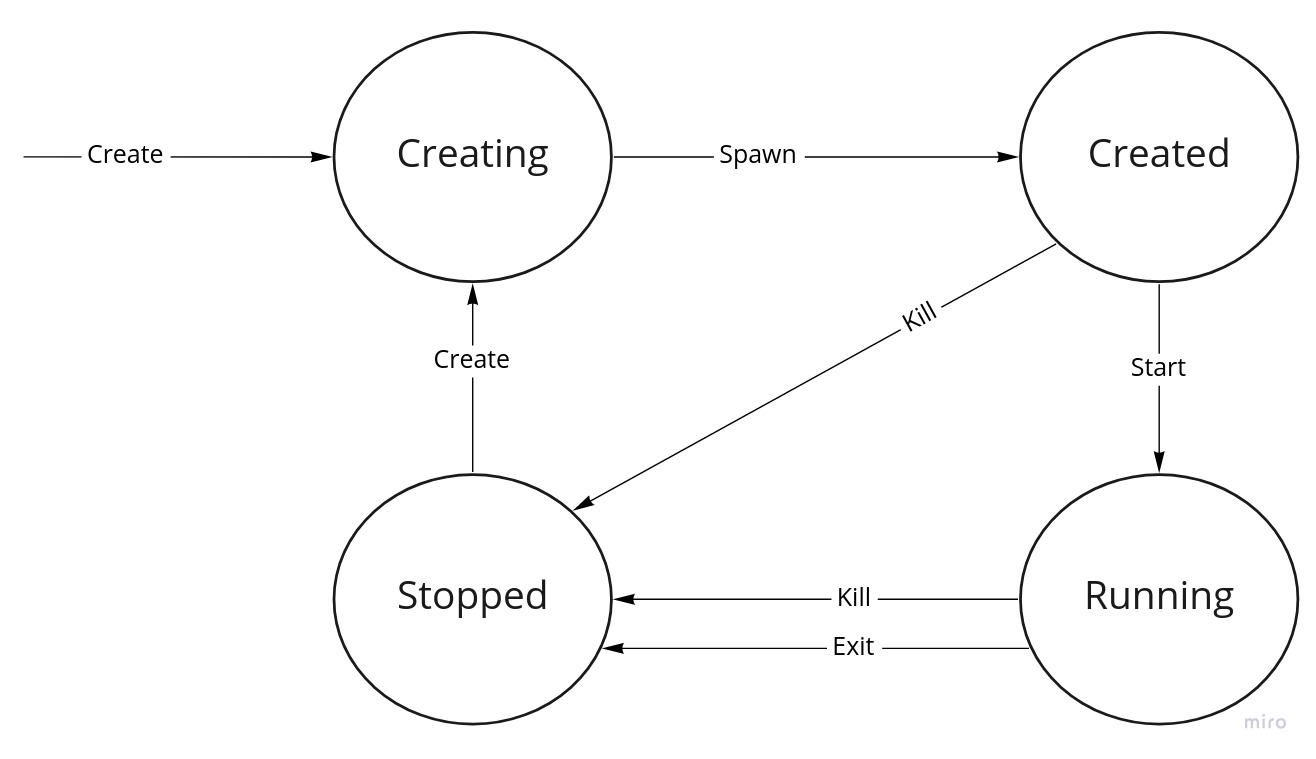
\includegraphics[width=0.5\textwidth]{images/concept/container-state-diagram.jpg}
    \caption{State transition diagram of container states. Every state transition is triggered by an operation, whose name is 
    specified in the arrow.}
    \label{images:concept/container-state-diagram.jpg}
\end{figure}

%\begin{table}[h!]
%    \centering
%    \begin{tabular}{ |m{3.5cm}|m{3.5cm}|m{20em}| }
%        \hline
%        Lifecycle Checkpoint & Request & Description \\
%        \hline
%        Runtime Creation & \verb|EVENT_RT_CREATE| & The container instructs the runtime to execute the runtime creation hooks on the host \\
%        \hline 
%        Container Creation & \verb|EVENT_CONT_CREATE| & The runtime instructs the container to execute the container creation hooks inside the container environment, after the runtime has been created \\
%        \hline 
%        Container Starting & \verb|EVENT_CONT_START| & The runtime instructs the container to execute the container start hooks inside the container environment, right before the user-defined binary is executed \\
%        \hline 
%        Container Started & \verb|EVENT_CONT_STARTED| & The container instructs the runtime to execute the container post-start hooks inside the runtime environment, right after the user-defined binary is executed \\
%        \hline 
%    \end{tabular}
%    \caption{Table of requests}
%    \label{table:concept/container-runtime/architecture/events}
%\end{table}

Every container has a dedicated root filesystem with its own set of device nodes,
pseudo filesystems, applications and libraries. The mount component in Figure \ref{images:concept/runtime-arch-overview.jpg}
atomically changes the container's root mount to a user-defined directory that holds its new root file system.
It then creates private mount points for all necessary pseudo filesystems, e.g \verb|proc|, \verb|sys|, and \verb|mqueue|. 
In addition, this component creates private device nodes for the container such as \verb|/dev/null| and \verb|/dev/urandom|.

The namespace component simply wraps some of the namespace system calls and provides a 
mechanism to enumerate a contiguous sequence of namespaces.

The clone component wraps the raw \verb|clone3()| system call and the \verb|glibc| wrapper 
into a portable (at least for \verb|x86_64| and \verb|aarch64|) set of functions.

The Open Containers Initiative (OCI) component is responsible for parsing a JSON configuration 
file that defines the container's execution environment. Code snippet \ref{code:oci-config.json} 
is an example of such a file. In addition, this component provides a mechanism for executing an 
arbitrary program, called a hook, that receives the container's state through its standard input stream as a JSON string.
Hooks are provided by external applications as part of the JSON configuration file and are executed
when a container transitions into a new state.  This design is defined as part of the runtime specification \cite{oci-runtime-lifecycle}. 
A container's state transition diagram is shown in Figure \ref{images:concept/container-state-diagram.jpg}.
Table \ref{table:concept/runtime/hooks} shows the predefined set of hooks and in which execution 
context they are executed.

\begin{table}[h!]
    \centering
    \begin{tabular}{ |c|c|c| }
        \hline
        Hooks & Namespace & Triggered By \\
        \hline
        \verb|on_runtime_create| & Runtime namespace & \verb|EVENT_RT_CREATE| \\ % & Prepare runtime environment on the host \\
        \hline 
        \verb|on_container_created| & Container namespace & \verb|EVENT_CONT_CREATE| \\ %& Prepare runtime environment inside the container, before pivoting the new root filesystem  \\
        \hline
        \verb|on_container_start| & Container namespace & \verb|EVENT_CONT_START| \\ % & Prepare runtime environment inside the container, after pivoting but before \verb|execve| \\
        \hline
        \verb|on_container_started| & Runtime namespace & \verb|EVENT_CONT_STARTED| \\ %& Run a set of post-start hooks on the host \\
        \hline
        \verb|on_container_stopped| & Runtime namespace & \verb|SIGCHLD| \\ %& Clean up runtime environment on host, after container has exited \\
        \hline
    \end{tabular}
    \caption{Table of hooks, where they are executed and what event they are triggered by.}
    \label{table:concept/runtime/hooks}
\end{table}

\begin{figure}[H]
    \centering
    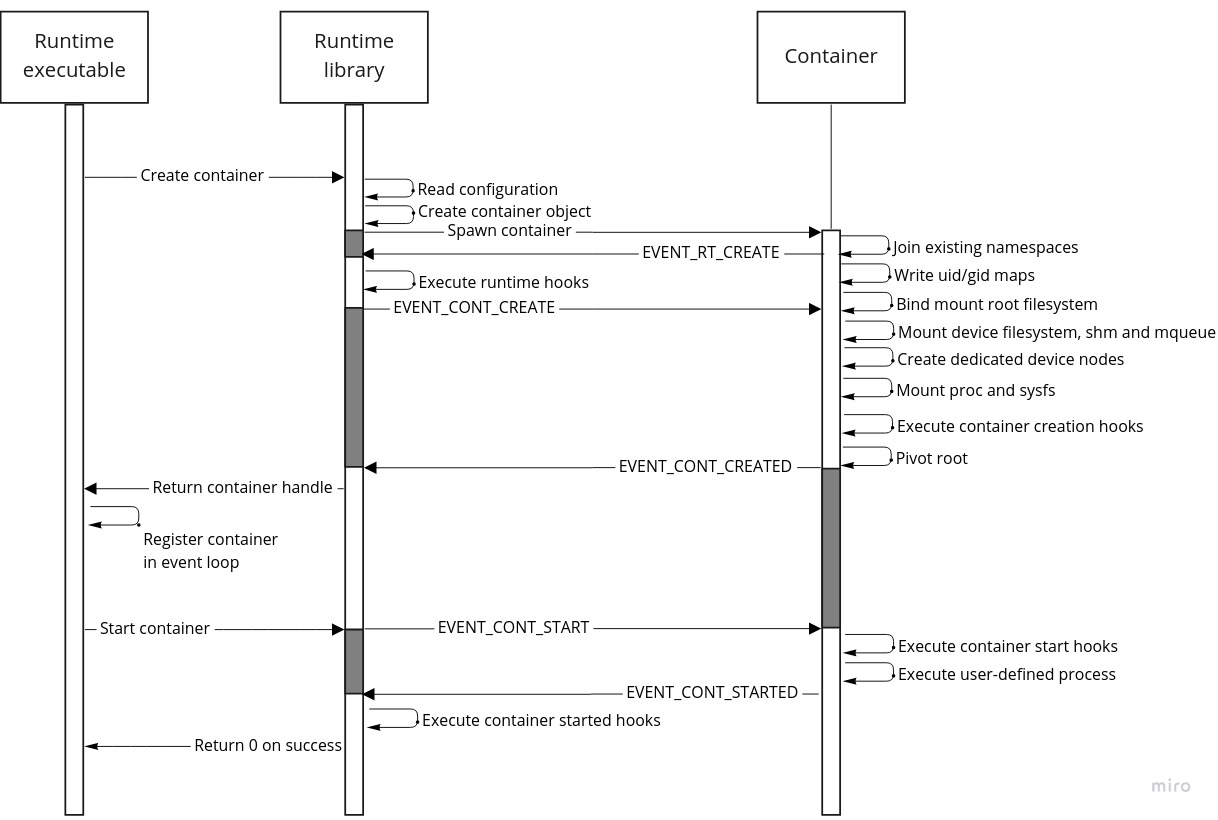
\includegraphics[width=0.8\textwidth]{images/concept/container-create-start-sequence-diagram.jpg}
    \caption{Sequence diagram highlighting the container creation and start operations}
    \label{images:concept/container-create-start-sequence-diagram.jpg}
\end{figure}

 The \verb|on_runtime_create| hooks are executed in the runtime namespace 
and prepare the runtime environment on the host. These hooks are triggered after the container process 
is cloned into a new set of namespaces. The \verb|on_container_created| hooks are executed within 
the container namespaces in order to prepare the runtime environment inside the container.
Note that these hooks are executed before the root filesystem is pivoted.
The \verb|on_container_start| hooks are triggered after pivoting the root filesystem, but before 
loading the user-defined application via \verb|execve()|. The \verb|on_container_started| hooks 
are executed within the runtime namespaces after the \verb|execve()| is called. 
The process is then monitored for state changes. Whenever it exits, the \verb|on_container_stopped|
hooks are executed, whose primary task is to clean up the runtime environment on the host. 

The synchronisation component defines an inter-process communication mechanism between 
the container runtime and a container. The typical communication flow follows the request-response pattern - 
one end produces a request and blocks until the other end consumes it and produces a response.
However, to enable concurrent work, a peer can \enquote{fire} a message and forget about the response.
The requests and responses are simple numeric values with semantic meaning. 

The container component brings all of the core components together. The sequence diagram in 
Figure \ref{images:concept/container-create-start-sequence-diagram.jpg} shows the procedures 
executed to create and start a container. The runtime executable invokes the create
operation, as defined in requirement (\ref{requirements:container-runtime/2}). 
The container component reads the configuration file and allocates 
an in-memory representation for the container. It then spawns the container process, which creates 
a freshly-allocated set of namespaces and joins already existing namespaces, depending on the namespace configuration 
specified in the file.

It then transitions into the \enquote{creating} state and notifies the runtime to execute the 
corresponding hooks by sending an \verb|EVENT_RT_CREATE| through the synchronisation component. 
The runtime receives the request, executes the runtime hooks, and notifies the child that it should transition 
into the \enquote{created} state by executing the container creation hooks and atomically swapping the old root mount 
with the new root filesystem. The container process then blocks indefinitely until it is killed 
or it receives a start request from the runtime executable. The latter will trigger yet another 
hook execution procedure, it will move the container into the \enquote{running} state and will afterwards run the user-defined binary. 
This is detected 
by the runtime, a set of post-start hooks is triggered, and the runtime executable is notified 
of the operation's completion.  

After the container is created, the executable is responsible for 
managing the container process. It does so by registering the container with an event loop that
polls container states and reaps processes that have terminated, which happens when the container 
transitions into the \enquote{stopped} state - either by exiting or being manually killed by the executable through 
a signal. 

%\begin{figure}[H]
%    \centering
%    \includegraphics[width=0.7\textwidth]{images/concept/runtime-create-start-kill-sequence-diagram.jpg}
%    \caption{Sequence diagram highlighting the interaction of a client application with the runtime executable.}
%    \label{images:concept/images/concept/runtime-create-start-kill-sequence-diagram.jpg}
%\end{figure}

%Figure \ref{images:concept/images/concept/runtime-create-start-kill-sequence-diagram.jpg} shows 
%the commands that an external application can send to the runtime executable. The application 
%creates a streaming socket and establishes a connection to the runtime server. 
%The runtime accepts the connection and registers the socket file descriptor with the event loop. 
%Whenever the client writes data into the socket, the runtime wakes up from the suspended state and reacts to the 
%event by parsing the request and processing it. When the client requests the creation 
%of a new container, by sending \verb|create <container-name> <config-path>|, 
%the runtime calls out to the library and registers the container in a hash table. Furthermore, 
%a pollable file descriptor for that container is created and registered with the event loop. 
%When the process exits, the kernel notifies the runtime of the event, so it can reap the process accordingly.
%The runtime is responsible for keeping the container's state machine consistent with the events 
%received from the kernel, as well as the requests that come from the client.

%The runtime uses the \verb|epoll| family of system calls to simultaneously monitor multiple file descriptors 
%to see if any I/O is possible on any of them. It also uses a new kernel application programming interface - 
%process file descriptors, commonly abbreviated as \verb|pidfd|'s, to map process identifiers to 
%pollable objects that can be registered with an event loop. All of these concepts are explained 
%in Chapter \ref{ch:implementation}.

\section{Benchmark}
Benchmarking is a tool to test performance in a controlled way, allowing different 
system and software configurations to be compared and analysed.

\subsection{Functional requirements}
\begin{enumerate}[i]
    \item The benchmark must facilitate the collection of performance metrics in native and containerised environments.
    \label{requirements:functional/benchmark/1} 
    \item The benchmark must aggregate and compare metrics in native and containerised environments to 
    enable the detection of isolation overheads.
    \label{requirements:functional/benchmark/2}
    \item The benchmark must produce observable results, either through visualisations or formatted text outputs,
    so that they can be analysed.
    \label{requirements:functional/benchmark/3}
    \item The benchmark must expose a command-line interface that allows users to define their own 
    container and sampling configurations.
    \label{requirements:functional/benchmark/4}
\end{enumerate}

\subsection{Workloads \& Metrics}
A workload is an application aimed at stressing a particular path of execution. 
Workloads are executed within an environment, e.g a container or on the host.
While the workload is running, a set of tracepoints accumulate performance counters relevant to that 
path of execution, which are then aggregated into statistics. 
The tracing procedures may be embedded in the workload itself, or as an external application. 

The tracepoints focus on building accurate representations of two variables - latency and throughput. 
The former is a measure of the time spent waiting for a particular resource. The latter 
is a measure of the number of operations than a resource can process per unit of time.
The benchmark tool, or the workload itself, attaches tracepoints to resources 
that are namespaced by the kernel and gathers information while the workload is running inside 
the container. Afterwards, the same statistics are gathered by executing the workload again, but this time 
as a native application absent of a noninterference boundary constructed by the container runtime. 
The difference in latency and throughput between both runs acts as an approximation of the isolation 
overhead introduced by sandboxing the workload. In Chapter \ref{ch:Experiment}, this approximation will be used 
to evaluate a set of hypotheses. 

In this section, the workloads and the performance counters associated with them are described. 

\subsubsection{Network workload}
\label{ch:concept/benchmark/net-workload}
The goal of this workload is to measure the overhead of data transmission between 
two separate network namespaces. The workload consists of a client and a server that communicate 
via TCP or UDP. Users have to specify the execution environment of both the client 
and the server. Hence, both can be deployed in two separate containers, each having a dedicated
virtual ethernet cable attached to a bridge device on the host that switches packets between them.
Alternatively, one of the components can run 
in the root network namespace, i.e directly on the host system. A third option is to have both 
the client and the server run on the host system without a bridge device between them. This is how 
native applications communicate - by being attached to the same network interface. 

The workload begins by starting the server and then the client. The client begins sending out as many 
data chunks of size $b$ as possible during equally-spaced intervals of $n$ seconds for a total 
duration of $t$ seconds.
During the data exchange procedure, the client keeps track of round-trip time, the number 
of bytes transfered, the bits transferred per second, and the number of retransmissions for each interval $n$. 
The caller configures $b$, $n$ and $t$. In additon, the caller is allowed to configure the number 
of parallel connections betwen the client and the server. In that case, the aforementioned 
statistics will be tracked for each connection. Increasing the number of connections can be used to
determine the degree of saturation, i.e how many connection are necessary to 
observe increases in latency and decreases in throughput due to throttling.
The workload also keeps a summary of the total user and system time it spends on the processing units,
both for the client and the server.

Note that the number of retransmissions and the round-trip time are metrics that are tracked only 
for TCP because they are intrinsic to the protocol implementation in order to detect data loss 
and retransmit packets accordingly. Conversely, UDP is unreliable and does not maintain such information. 
Lost data and out of order packets must be handled at the application level.

Round-trip time is this workload's latency metric. 
It is an approximation of the amount of time it takes to send a packet 
to the server plus the time it takes to receive the acknowledgement of that packet. 
The round-trip time is a value maintained by the kernel's TCP implementation.
The number of bytes transferred during the interval is this workload's throughput metric.
It shows how much data can be forwarded from one network namespace to another via the bridge
and its slave devices. This value is accumulated in user-space, whenever the \verb|read()| system call 
finishes on the receiver's end the counter is incremented.
The number of retransmissions acts as a robustness metric for the network itself.
It also has a statistical relationship with throughput.
Higher retransmission counts may have a negative impact on throughput.

\subsubsection{Filesystem workload}
The purpose of this workload is to detect and analyse differences in latency and throughput in 
different mount namespaces. In particular, we want to compare these metrics when running the 
workload within the root mount namespace and a container mount namespace. 

The workload executes operations on a single file. Users can define the I/O pattern issued to the file,
e.g performing only sequential reads, writing to the file at random file offsets, using direct I/O
in order to bypass the page cache and so on. In addition, the size of the buffers (the block size)
can be configured. How the workload should issue the I/O operations must also be specified. 
There are a plethora of options here. I/O operations can be synchronous, i.e employing calls to 
\verb|read()|, \verb|write()| and \verb|lseek()| to 
position file offsets. Alternatively, I/O operations can be asynchronous. That is, 
the workload registers a set of event handlers for each I/O operation it wants to execute and only 
submits requests to the kernel. The kernel does not block the calling thread. Instead,
it notifies the application whenever the disk driver emits an interrupt that represents 
the operation's completion. In asynchronous mode, users can configure the number of parallel 
I/O operations. Another way of controlling parallelisation is by spawning multiple processes that 
compete with each other. The number of processes is also configurable.

Input-output operations per second (IOPS) is this workload's throughput metric.
The metric is heavily dependant on the I/O pattern employed. 
This work focuses on sequential reads and writes, both in synchronous and asynchronous contexts.
For the asynchronous measurements, the number of in-flight I/O operations is controlled by 
two mechanisms - number of processes issuing I/O operations and number of parallel I/O operations 
by a single process. These mechanisms are used independently to ease the interpretation of the results.
For the synchronous measurements, the level of parallelisation is controlled only through the number 
of processes.

Total latency is this workload's latency metric. The total latency is derived by summing 
two variables - the submission latency and the completion latency. The former represents 
the time it takes to allocate and initialise the data buffers plus a variable $a$ whose interpretation 
depends on whether or not the underlying I/O mechanism is synchronous or not.  
If it is, then $a = 0$. Otherwise, $a$ includes the time it takes to submit the I/O operation
to the underlying queue of requests. The completion latency is also context-dependant. 
In the synchronous case, it represents the time from when the input-output operation was submitted 
to the kernel to when it was completed. In the asynchronous case, it is the time from 
when the submission operation was completed to when the event handler that reaps the operation 
was completed. Intuitively, synchronous operations exhibit lower submission latencies but higher 
completion latencies. Conversely, asynchronous operations exhibit higher submission latencies 
but lower completion latencies. Completion latencies have a stronger impact on overall 
I/O performance, making asynchronous mechanisms more favorable for performance-critical workloads.    \clearpage
\chapter{Implementation}
\label{ch:implementation} \clearpage
\chapter{Results}
\label{ch:results} \clearpage
\chapter{Conclusion}
\label{ch:conclusion}
The results presented in the previous chapter show that the isolation overhead 
of process containerisation through resource namespacing is negligible. Disk latencies and throughput measurements 
in containers are on par with the same measurements on the host.
The networking infrastructure required to enable inter-container communication may lead to 
packet loss, higher retransmission counts and therefore increased latencies and decreased throughput.
Nevertheless, the average latency and throughput over the lifespan of a workload are almost
equivalent to running the application on the host. Furthermore, it is shown that 
hardware virtualisation mechanisms impact the resulting latencies and throughput far more 
severely \cite{https://doi.org/10.1002/cpe.5693} \cite{8457798}.
From a business perspective, the near-native performance of containers makes them highly 
favourable for consolidating multiple applications on a single server. The primary 
challenges with containers, however, lie not in performance, but rather security.

\section{Discussion}
Resource namespaces encapsulate a variety of kernel resources, but not all of them.
Namespace-unaware kernel subsystems resort to authorising operations with the user identifiers 
in the root user namespace, i.e those that were mapped by the container runtime into the container.
Containers that share these identifiers implicitly share various in-kernel data structures 
that may lead to interference. For example, the kernel used to (up to v5.13.19) impose per-user resource consumption 
restrictions such as the total number of file descriptors that can be kept open by that user, the number of 
pending signals that can be queued among all processes of that user, and the number of processes 
that the user can spawn. If one container exhausts these limits, other containers poentially owned by a different tenant are directly affected, i.e 
interfered with. This particular problem has been fixed in the v5.14 release by binding resource limit counters to user namespaces
\cite{https://patchwork.kernel.org/project/linux-hardening/cover/cover.1619094428.git.legion@kernel.org/}.
Another very important example are filesystem implementations. Filesystems associate every file 
with a unique user identifier that is its owner. Root filesystems for containers residing on the 
host are typically owned by a single user and group (allocated by the container engine) and are inaccessible by other users 
to prevent tampering. Hence, to meaningfully mount such a filesystem in multiple rootless containers, 
each container's identifier map must point to that user on the host, i.e all containers must 
share the same user identifier. This problem has been tackled by traversing the entire directory hierarchy and changing the 
ownership of each node to the root user within the container after the mount - an error-prone operation 
that can take approximately 40 seconds for a large enough root filesystem \cite{https://github.com/containerd/containerd/pull/4734}.
Not only is this operation slow, but it affects the ownership values on the host system, thereby necessitating that 
containers with different identifier mappings must have a dedicated copy of their root filesystem, which wastes storage.
This is the primary reason that rootless containers have not gained widespread adoption.
The problem was addressed in v5.12 by allowing user-space processes to associate an identifier mapping with every mount point \cite{https://lwn.net/Articles/896255/} through 
a new system call \verb|mount_setattr()|.
This identifier mapping is used to translate the caller's user identifier to the filesystem user identifier in a 
localised way \cite{https://www.kernel.org/doc/html/latest/filesystems/idmappings.html}.
In general, both examples above show that kernel developers are actively working on hardening 
the noninterference boundary and supporting container software in user-space.

\section{Future work}
This work can be further improved in two areas - the implementation of the container runtime 
and the benchmarking tool. The former is discussed first. 
The current implementation of the runtime does not incorporate the kernel's capability
framework, which allows for fine-grained control over the container's capability sets.
Another unsupported (and very important) feature
is resource control groups, also referred to as \textit{cgroups}. Resource control groups 
are a feature in the kernel that primarily deals with temporal noninterference. It is responsible 
for restricting the usage of various resources, such as processing units, memory and disk
to prevent denial of service attacks. Properly configuring control groups without degrading
application performance is a nuanced challenge that, in the 
authors opinion, is an interesting topic for a thesis.
Another innovative technology in the kernel is the eBPF subsystem, which allows 
for user-space programs to safely inject source code into arbitrary points in the kernel
and sample data. This technology can be integrated within the runtime, e.g for sampling 
behavior data of containerised processes and acting upon it, e.g if malicious intents are detected. 
The benchmark tool can also utilise eBPF for creating custom performance statistics. \clearpage
\chapter{Appendix A}
\section{Hardware Virtualisation}
\label{ch:fundamentals/virtualisation/hardware-virtualisation}
\textcite{10.1145/361011.361073} refer to the control program as a \textit{virtual machine monitor} that 
ensures isolation and noninterference by providing every program with an environment that is \enquote{[...] effect
identical with that demonstrated if the program had been run on the original machine directly} 
\cite[2]{10.1145/361011.361073}. This definition implies that a running program does not directly use
the bare metal resources available. Instead, resources are emulated by the virtual machine monitor at
the hardware level and presented as a dedicated physical system. Such an environment is called 
a \textit{virtual machine}.

\begin{figure}[H]
    \centering
    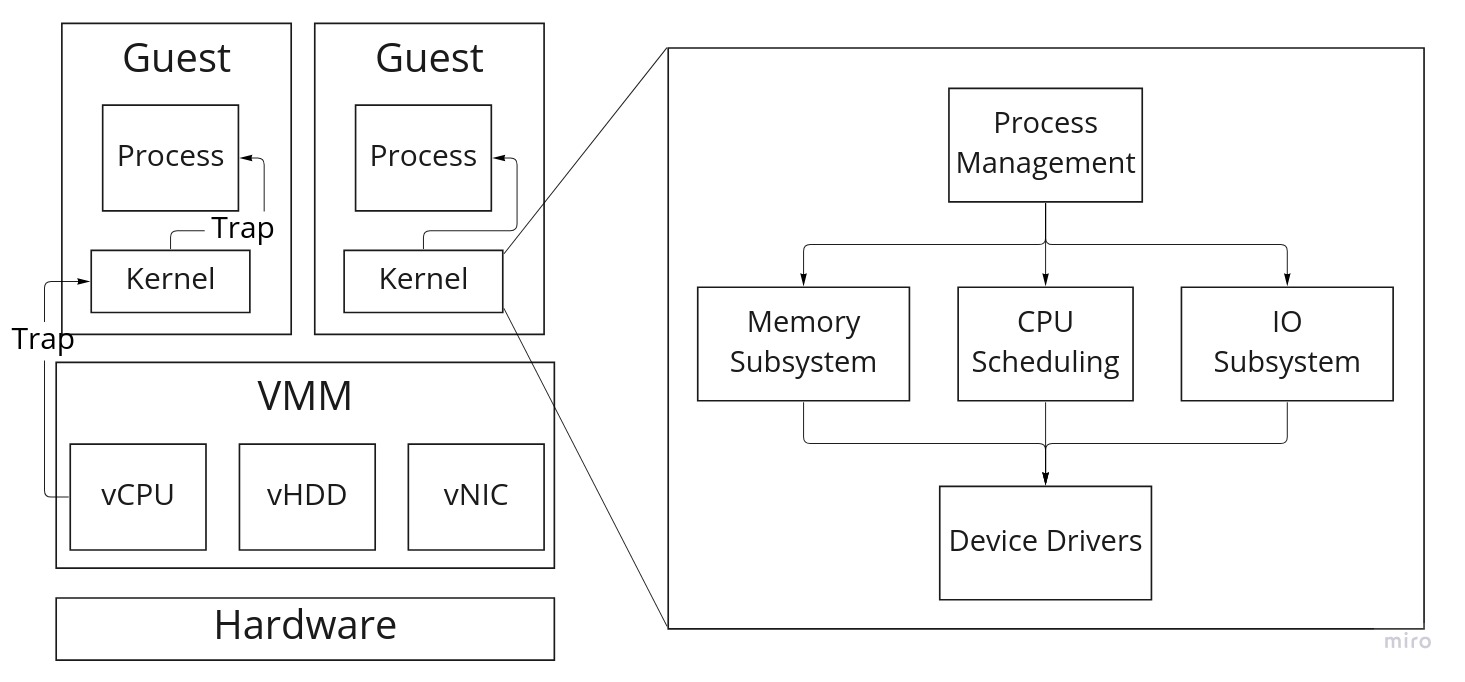
\includegraphics[width=0.70\textwidth]{images/fundamentals/full-virt-archh.jpg}
    \caption{Hardware virtualisation architecture. Each guest runs a complete operating system. 
             Privileged operations are trapped by the virtual machine monitor and emulated to provide hardware services.}
    \label{images:fundamentals/full-virt-archh.jpg}
\end{figure}

\textcite{10.1145/361011.361073} define a requirement that the instruction-set architecture of a computer
has to satisfy for it to be virtualisable. The instruction set must be segregated into three groups of
instructions - privileged, sensitive and innocuous. An instruction is privileged if it requires changing
the mode of execution from user to supervisor mode by means of a trap \cite{10.1145/361011.361073}. 
An instruction $i$ is control-sensitive if, when applied to the current processor state $S_1$, results
in a new state $i(S_{1}) = S_{2}$ such that the execution mode of $S_{2}$ does not equal that of $S_{1}$
or if $S_{2}$ has access to different resources than $S_1$ or both \cite{10.1145/361011.361073}. 
An instruction is behaviour-sensitive if its execution depends on the execution mode or its position
in memory \cite{10.1145/361011.361073}. An instruction is innocuous if it is not sensitive. 
Given these definitions, a computer is virtualisable \enquote{[...] if the set of sensitive instructions
for that computer is a subset of the set of privileged instructions} \cite[6]{10.1145/361011.361073}.
If this criterion is met, the virtual machine monitor can trap all sensitive instructions and emulate 
each via a homomorphism $i: C_{r} \rightarrow C_{v}$ that maps the state space of the processor without
the virtual machine monitor loaded $C_{r}$ to the state space with the virtual machine monitor loaded 
$C_{v}$ \cite{10.1145/361011.361073}. Innocuous instructions do not require protection, i.e a homomorphic
mapping, and are directly executed by the processor \cite{10.1145/361011.361073}.

Given the aforementioned homomorphism, a virtual machine can host a \textit{guest kernel} (Figure \ref{images:fundamentals/full-virt-archh.jpg}) that 
runs completely in user mode. 
Whenever the guest kernel attempts to execute a privileged instruction, 
the virtual machine monitor traps the attempt and emulates the instruction. 
Consequently, the guest kernel does not have to be a part of the trusted computing base. 
Even if it is compromised or encounters an unrecoverable error condition, other virtual machines 
remain unaffected. As a result, the isolation boundary between user programs running in different 
virtual machines is stronger compared to processes running on a shared kernel. 

In order to fully guarantee spatial noninterference between processes, the virtual machine monitor must 
be in full control of the host system's memory. There are two primary methods to do this - 
\textit{shadow paging} and \textit{extended page tables}. The former mechanism is considered first. 
The virtual machine monitor maintains a nested page table 
per guest, also called a \textit{shadow page table} \cite{10.5555/1204009}. 
In turn, the guest kernel maintains a page table per process. 
Whenever the guest kernel schedules a new process for execution, it modifies the \textit{page-table 
base register} to point to the page table for that process \cite{10.5555/1204009}. 
The virtual machine monitor intercepts this attempt and transparently updates the page table pointer to point to 
the guest's shadow page table corresponding to that process \cite{10.5555/1204009}. Note that 
the virtual machine monitor has to traverse the shadow page table for that guest in order to find the nested entry corresponding 
to the process. Afterwards, the memory management unit takes care of translating the virtual memory 
addresses of the guest and updating the \textit{translation lookaside buffer}.
Alternatively, the memory management unit may be \enquote{virtualisation-aware} in the sense that it knows 
there are two page tables it needs to traverse - the page table that maps guest virtual memory to guest 
\enquote{physical memory}, and the page table that maps guest physical memory to actual physical memory. 
The former is maintained by the guest kernel, whilst the latter is maintained by the virtual machine monitor.
The extended page table approach is up to 50\% faster than shadow paging \cite{2006PerformanceEO} because table
walks are done in hardware - by the memory management unit.
Nevertheless, maintaining page table data structures inside the virtual machine 
monitor and the guests leads to memory pressure, which is further amplified by the fact that 
guests, their applications and the virtual machine monitor all share the same physical memory \cite{10.5555/2490781}. 

The spatial noninterference property necessitates that the virtual machine monitor manage 
all input-output devices and their interactions with the guests. This is accomplished by the
already introduced trap-and-emulate pattern. When an application within a virtual machine 
issues a system call requesting some form of input-output, the request is processed by the 
I/O stack inside the guest. At the lowest level of the stack, the device driver issues a 
command to the device, typically by writing to memory specifically assigned to the device, or by
calling specific input-output instructions \cite{10.5555/2490781}. 
Either way, the virtual machine monitor intercepts this and traverses its own I/O stack, which 
remaps guest and real input-output addresses and forwards the request to a physical device \cite{10.1145/2063176.2063194}. 
After processing the request, the physical device triggers an interrupt that is caught by the virtual machine monitor and 
transformed into a virtual equivalent that is sent to the virtual machine that issued the request.
To reduce the overhead associated with interrupt processing, the virtual machine monitor can batch 
multiple events together and use a single interrupt to notify the guest kernel \cite{10.1145/2063176.2063194}.
Still, a request must traverse two input-output stacks. The same holds for the response.
In addition, hardware optimisations such as direct memory access are emulated in software, which 
further degrades performance. This, however, can be mitigated by integrating an input-output memory management 
unit that remaps all direct memory accesses of a device on the host to an address space in the guest.

The cost of hardware virtualisation becomes apparent when measuring same-host density
and boot times. \textcite{10.1145/3132747.3132763} consider memory consumption and on-disk image size
as the primary limiting factors. The authors measure the time it takes to create and boot
virtual machines using the Xen virtual machine monitor and show the negative effects that on-disk image size has 
by starting images with 
varying sizes by manually \enquote{[...] injecting binary objects into the uncompressed image file} \cite[3]{10.1145/3132747.3132763}. 
As the number of consolidated virtual instances increases and the image size grows, 
creation and boot times increase linearly.
Furthermore, the authors show that creating and starting a process directly on the host is, on average, 
two orders of magnitude faster. \textcite{10.1145/2151024.2151030} also evaluate Xen and state
that processing units spend 25\% of their total cycles in hypervisor mode instead of executing guest applications 
when running \enquote{[...] SPEC's first benchmark addressing performance evaluation of datacenter servers used in 
virtualised server consolidation} \cite[2]{10.1145/2151024.2151030}, which includes components 
such as a web, database and application server.

\section{Container configuration}

\begin{lstlisting}[style={syscalls}, label={code:oci-config.json}, caption={Open Containers Initiative Configuration File Example}]
{
    "process": {
        "args": [
        "nsbench-disk-workload"
        ],
        "cwd": "/"
    },
    "root": {
        "path": "./workloads/rootfs/disk",
        "readonly": false
    },
    "namespaces": [
        {
        "type": "user"
        },
        {
        "type": "net"
        },
        {
        "type": "ipc"
        },
        {
        "type": "mnt"
        },
        {
        "type": "uts"
        },
        {
        "type": "pid"
        }
    ],
    "uid_mappings": [
        {
        "container_id": 0,
        "host_id": 1000,
        "size": 1
        }
    ],
    "gid_mappings": [
        {
        "container_id": 0,
        "host_id": 1000,
        "size": 1
        }
    ],
    "hostname": "nsbench-disk-workload",
    "hooks": { 
        "on_runtime_create": [
            {
                "path": "/usr/bin/setup-network",
                "args": ["-a", "192.168.0.101"],
                "env": ["PATH=/usr/bin"],
                "timeout": 2
            }
        ],
        "on_container_created": [],
        "on_container_start": [],
        "on_container_started": [],
        "on_container_stopped": []
    }
}
\end{lstlisting}

\begin{lstlisting}[style=c-code-snippets, label={code:implementation/benchmark/network-hook-doer}, caption={Joining an arbitrary namespace, executing a function within it, and returing back to the original namespace}]
func DoInContainerNamespace(containerPid, namespace int, doer func() error) error {
    runtime.LockOSThread()
    defer runtime.UnlockOSThread()

    ns, ok := namespaces[namespace]
    if !ok {
        return ErrNamespaceUnsupported
    }

    oldNsPath := path.Join("/proc", "self", "ns", ns)
    oldNsFd, err := unix.Open(oldNsPath, unix.O_RDONLY|unix.O_CLOEXEC, 0)
    if err != nil {
        return err
    }
    defer unix.Close(oldNsFd)

    newNsPath := path.Join("/proc", strconv.Itoa(containerPid), "ns", ns)
    newNsFd, err := unix.Open(newNsPath, unix.O_RDONLY|unix.O_CLOEXEC, 0)
    if err != nil {
        return err
    }
    defer unix.Close(newNsFd)
    if err := unix.Setns(newNsFd, namespace); err != nil {
        return err
    }
    defer unix.Setns(oldNsFd, namespace)
    return doer()
}
\end{lstlisting}

\section{Netlink protocol}
\label{ch:appendix/netlink-protocol}

\clearpage
%\input{chapter/Analysis} \clearpage
%\input{chapter/Conception} \clearpage
%\input{chapter/Implementation} \clearpage
%\input{chapter/Test} \clearpage
%\input{chapter/Evaluation} \clearpage
%\input{chapter/Conclusion} \clearpage

\pagenumbering{Roman}
% List of Figures
\listoffigures \clearpage
% List of Tables
\listoftables \clearpage
% Source Code Content
\lstlistoflistings \clearpage

\printindex \clearpage

\printnoidxglossary[title=Glossar] \clearpage

\defbibfilter{scientific}{
	type=article or
	type=inbook or
	type=book or
	type=unpublished or
	type=inproceedings or
	type=incollection or
	type=manual or
	type=phdthesis
}

\printbibliography[heading=bibintoc, filter=scientific, title={References}]\clearpage
\printbibliography[heading=bibintoc, keyword={online}, title={Online References}]\clearpage
\printbibliography[heading=bibintoc, keyword={image}, title={Image References}]\clearpage

\end{document}
